\documentclass[cs4size,a4paper]{ctexart}   
%==================== 数学符号公式 ============
%!TEX program = xelatex

\usepackage{amsmath}                 % AMS LaTeX宏包
\usepackage[style=1]{mdframed}
\usepackage{amsthm}
\usepackage{amsfonts}
\usepackage{mathrsfs}                % 英文花体字 体
\usepackage{bm}                      % 数学公式中的黑斜体
\usepackage{bbding,manfnt}           % 一些图标,如 \dbend
\usepackage{lettrine}                % 首字下沉,命令\lettrine
\def\attention{\lettrine[lines=2,lraise=0,nindent=0em]{\large\textdbend\hspace{1mm}}{}}
\usepackage{longtable}
\usepackage[toc,page]{appendix}
\usepackage{geometry}                % 页边距调整
\geometry{top=3.0cm,bottom=2.7cm,left=2.5cm,right=2.5cm}
%====================公式按章编号==========================
\numberwithin{equation}{section}
\numberwithin{table}{section}
\numberwithin{figure}{section}
%================= 基本格式预置 ===========================
\usepackage{fancyhdr}
\pagestyle{fancy}
\fancyhf{}  
\fancyhead[C]{\zihao{5}  \kaishu 简明全球史}
\fancyfoot[C]{~\zihao{5} \thepage~}
\renewcommand{\headrulewidth}{0.65pt} 
\CTEXsetup[format={\centering\bfseries\zihao{-2}},name={第, 章}]{section}
\CTEXsetup[nameformat={\bfseries\zihao{3}}]{subsection}
\CTEXsetup[nameformat={\bfseries\zihao{4}}]{subsubsection}
%================== 图形支持宏包 =========================
\usepackage{subfigure}
\usepackage{graphicx}                % 嵌入png图像
\usepackage{color,xcolor}            % 支持彩色文本、底色、文本框等
\usepackage{hyperref}                % 交叉引用
\usepackage{caption}
\captionsetup{figurewithin=section}
%==================== 源码和流程图 =====================
\usepackage{listings}                % 粘贴源代码
\usepackage{xcolor}
\usepackage{color}
\definecolor{dkgreen}{rgb}{0,0.6,0}
\definecolor{gray}{rgb}{0.5,0.5,0.5}
\definecolor{mauve}{rgb}{0.58,0,0.82}
 \usepackage{xcolor}
 \lstset{
  %行号
    numbers=left,
    %背景框
    framexleftmargin=8mm,
    frame=none,
     %背景色
    %backgroundcolor=\color[rgb]{1,1,0.76},
     backgroundcolor=\color[RGB]{245,245,244},
     %样式
   keywordstyle=\bf\color{blue},
   identifierstyle=\bf,
    numberstyle=\color[RGB]{0,192,192},
    commentstyle=\it\color[RGB]{0,96,96},
   stringstyle=\rmfamily\slshape\color[RGB]{128,0,0},
   %显示空格
    showstringspaces=false
 }


%--------------------
\hypersetup{hidelinks}
\usepackage{booktabs}  
\usepackage{shorttoc}
\usepackage{tabu,tikz}
\usepackage{float}

\usepackage{multirow}



\tabcolsep=1ex
\tabulinesep=\tabcolsep
\newlength\tikzboxwidth
\newlength\tikzboxheight
\newcommand\tikzbox[1]{%
        \settowidth\tikzboxwidth{#1}%
        \settoheight\tikzboxheight{#1}%
        \begin{tikzpicture}
        \path[use as bounding box]
                (-0.5\tikzboxwidth,-0.5\tikzboxheight)rectangle
                (0.5\tikzboxwidth,0.5\tikzboxheight);
        \node[inner sep=\tabcolsep+0.5\arrayrulewidth,line width=0.5mm,draw=black]
                at(0,0){#1};
        \end{tikzpicture}%
        }

\makeatletter
\def\hlinew#1{%
  \noalign{\ifnum0=`}\fi\hrule \@height #1 \futurelet
   \reserved@a\@xhline}
   
\newcommand{\tabincell}[2]{\begin{tabular}{@{}#1@{}}#2\end{tabular}}%

\usepackage{subfigure}

\usepackage{CJK}
\usepackage{ifthen}


\usepackage{graphicx} 
\newcommand{\HRule}{\rule{\linewidth}{0.5mm}}

\newtheorem{Theorem}{定理}
\newtheorem{Lemma}{引理} 
%%使得公式随章节自动编号
\makeatletter
\@addtoreset{equation}{section}
\makeatother
\renewcommand{\theequation}{\arabic{section}.\arabic{equation}}

%-------------------------
	
\usepackage{pythonhighlight}
\usepackage{tikz}                    
\usepackage{tikz-3dplot}
\usetikzlibrary{shapes,arrows,positioning}
%===================   正文开始    ===================
\begin{document}
\bibliographystyle{gbt7714-2005}     %论文引用格式
%===================  定理类环境定义 ===================
\newtheorem{example}{例}              % 整体编号
\newtheorem{algorithm}{算法}
\newtheorem{theorem}{定理}            % 按 section 编号
\newtheorem{definition}{定义}
\newtheorem{axiom}{公理}
\newtheorem{property}{性质}
\newtheorem{proposition}{命题}
\newtheorem{lemma}{引理}
\newtheorem{corollary}{推论}
\newtheorem{remark}{注解}
\newtheorem{condition}{条件}
\newtheorem{conclusion}{结论}
\newtheorem{assumption}{假设}
%==================重定义 ===================
\renewcommand{\contentsname}{目录}     
\renewcommand{\abstractname}{摘要} 
\renewcommand{\refname}{参考文献}     
\renewcommand{\indexname}{索引}
\renewcommand{\figurename}{图}
\renewcommand{\tablename}{表}
\renewcommand{\appendixname}{附录}
\renewcommand{\proofname}{证明}
\renewcommand{\algorithm}{算法} 
%============== 封皮和前言 =================
\begin{titlepage}

\begin{center}


% Upper part of the page
%\includegraphics[width=0.65\textwidth]{figure/logo}\\[1cm]    

\textsc{\LARGE Concise world history}\\[1.5cm]

\textsc{\Large 第一版}\\[0.5cm]


% Title
\HRule \\[0.4cm]
{ \huge \bfseries 简明世界史}\\[0.4cm]

\HRule \\[1.5cm]

% Author and supervisor
% \begin{minipage}{0.4\textwidth}
% \begin{flushleft} \large
% \emph{Author:}\\
% 乔 \textsc{旭}
% \end{flushleft}
% \end{minipage}


% \begin{minipage}{0.4\textwidth}
% \begin{flushright} \large
% \emph{Supervisor:} \\
% Dr 芦翔 %\textsc{Bro}
% \end{flushright}
% \end{minipage}

\vfill

% Bottom of the page
{\large \today}

\end{center}

\end{titlepage}


%%=============设计(论文)任务书===========
%\begin{center}
%\zihao{-2}\textbf{\songti 本科生毕业设计(论文)任务书} 
%\end{center}
%\smallskip
%\renewcommand{\arraystretch}{1.3}
%\begin{tabular}{lll}
%\zihao{4} \textbf{\songti 学生姓名: 曹宇} & & \zihao{4} \textbf{\songti 专业班级:\quad\quad 船海1006班} \\ 
%\zihao{4} \textbf{\songti 指导教师:徐海祥}&\makebox [3cm] & \zihao{4} \textbf{\songti 工作单位:\quad 武汉理工大学} \\ 
%\end{tabular}\\
%\begin{tabular}{lll}
%\zihao{4} \textbf{\songti 设计(论文)题目:}& \zihao{4} \textbf{\songti  武汉理工本科论文\LaTeX 模板 } &\\ 
%\zihao{4} \textbf{\songti 设计(论文)主要内容:} \\
%\end{tabular} \\ 
%\begin{enumerate}
%\item \LaTeX 环境的配置
%\item 主要字体的控制和数学公式的选用
%\item 图表和代码的粘贴
%\end{enumerate}
%\begin{tabular}{ll}
%\zihao{4} \textbf{\songti 要求完成的主要任务:}
%\end{tabular} \\ 
%\begin{enumerate}
%\item 选择合适的\TeX 编辑系统
%\item 学习如何使用控制代码完成排版
%\item 合理的安排学习和科研的时间来发展自己兴趣爱好
%\end{enumerate}
%\begin{tabular}{ll}
%\zihao{4} \textbf{\songti 必读参考资料:}
%\end{tabular}
%\begin{enumerate}
%\item \LaTeX  \quad User Manual
%\item  字体设计的艺术
%\end{enumerate}
%\begin{tabular}{lll}
%\zihao{4} \textbf{\songti 指导教师签名: }&\makebox [4cm]& \zihao{4} \textbf{\songti 系主任签名:} \\
%& & \zihao{4} \textbf{\songti 院长签名(章)}
%\end{tabular}
%\thispagestyle{empty}
%\clearpage
%%==========本科生毕业设计(论文)开题报告  =============
%\begin{center}
%\zihao{-2} \textbf{\songti 武汉理工大学}\\
%\zihao{-2} \textbf{\songti 本科生毕业设计(论文)开题报告} 
%\end{center}
%\begin{tabular}{|l|}
%\hline \rule[-2ex]{0pt}{5.5ex} \makebox[13.5cm][l]{\zihao{4} \heiti 1、目的及意义(含国内外的研究现状分析) } \\ 
%\quad \LaTeX 是国际通行的科技论文排版软件,国际上科研机构和大学都采用它写作\\
%\quad 国内著名高校都有自己的本科生\LaTeX 模板供毕业生使用\\
%\quad 但是武汉理工大学还没有本科生\LaTeX 模板可以参考\\
%\quad 人类的价值在于创造而不是索取 \\
%\hline \rule[-2ex]{0pt}{5.5ex}  \zihao{4} \heiti
%2、基本内容和技术方案\\ 
%\quad 采用GITHUB托管降低代码维护成本\\
%\quad 加入在线\TeX 编辑器的使用简介 \\
%\quad 授人以渔,注重方法和理念的引导\\
%\hline \rule[-2ex]{0pt}{5.5ex}  \zihao{4} \heiti
%3、进度安排 \\ 
%\quad 离 deadline 两个月吃喝玩乐 \\
%\quad 离 deadline 一个月吃喝玩乐 \\
%\quad 离 deadline 半个月吃喝玩乐 \\
%\quad 离 deadline 一个星期狂写论文 \\
%\hline \rule[-2ex]{0pt}{5.5ex} \zihao{4} \heiti
%4、指导教师意见 \\ 
%\quad 曹宇同学是个好同志\\
%\quad 曹宇同志是个好同学\\
%\quad 本表格是支持跨页的长表格,你可以复制上面的内容进行测试\\
%\quad 具体方法是将tabular改为 longtable然后再编译\\
%\makebox[10cm][r]指导教师签名:\\
%\makebox[12cm][r]\quad 年\quad 月\quad 日\\
%\hline 
%\end{tabular} 
%\thispagestyle{empty}

\pagestyle{plain}
\pagenumbering{Roman}
% \section*{\zihao{2} \centering 摘要}

% \vskip0.5cm
% 本文主要基于国外已有的针对铱星通信链路解析的开源工程,展开进一步的分析。主要研究对象是铱星SBD通信方式。旨在通过对其已有的工具链进行分析和优化,实现针对该通信方式上行链路的解析。


% \textbf{关键词:}  铱星,通信链路分析,SBD通信,协议逆向
% \addcontentsline{toc}{section}{摘要}

% %\clearpage
% \section*{\zihao{2} \centering \textbf{Abstract} }
%   %用了Times New Roman字体来美化观感

% This article is mainly based on the existing open source projects for the analysis of Iridium communication links, and further analysis. The main research object is the comet SBD communication method. The aim is to analyze and optimize the existing toolchain to achieve the resolution of the uplink for this communication method.

% \textbf{Key Words:} Iridium, communication link analysis, SBD communication, protocol reverse
% \addcontentsline{toc}{section}{Abstract}





\pagestyle{empty}
\tableofcontents 
\thispagestyle{empty}
%============== 论文正文   =================
\pagestyle{fancy}
\pagenumbering{arabic}
\section{早期人类社会}
\subsection{人类起源}
地球发展的初期阶段时60亿年之前,46亿年前形成了地壳。从那时起,地球历史分为五个代:
\begin{enumerate}
    \item 太古代(约46亿年~25亿年)
    \item 元古代(约25亿年~6亿年)
    \item 古生代(约6亿年~2.25亿年)
    \item 中生代(约2.25亿年~7000万年)
    \item 新生代(约7000万年~至今)
\end{enumerate}

每一代分为若干纪,每纪分为若干世。

人类的进化过程大约是从森林古猿到南方古猿,直立人,早期智人(尼安德特人)再到晚期智人。至此出现了现代人种。

\subsection{旧石器时代的采集狩猎者}
% 为什么称之为旧石器时代?
% 采集狩猎者是什么鬼?
% 这一时代的特点是什么?

旧石器时代大体可以分为三个时期,分别为早期,中期和晚期。早期相当于最早的人属和直立人阶段,此时人类已经开始学会使用火。中期相当于早期智人阶段。晚期相当于晚期智人阶段。

在旧石器时代,人类主要使用石器为工具,石器制作技术在不同阶段逐渐成熟,在旧石器时代早期人类已能用火。

旧石器时代的人类以采集天然产物为主,如果实,块根,昆虫灯,同时也进行狩猎活动。采集和狩猎成为这个时代主要的劳动分工。火的使用在很大程度上加快了人类适应自然的进程,人类使用火种来进行御寒,保护自己,进而扩大了自己的活动范围。在晚期还出现了骨针,说明人们已经开始缝制衣服御寒。

生产技术的进步和生存条件的改善,导致了人类活动范围的扩大,人类开始向美洲及澳洲迁徙。大多数历史学家同意,人类通过东北亚的白令海峡的大陆桥进入美洲,此时正处于冰河时期,海平面降低。

\subsection{新石器时代的农业革命}
% 什么时间,发生了什么事
% 什么是新石器时代啊?
% 为什么认为是农业革命?
% 起因是什么?

从旧石器时代到新石器时代存在一段过渡时期,约15000年,从这时起,人类的经济活动有了进一步的发展。

同时,在中世纪时代,全球气候和生态环境发生显著变化。冰川期过去,全球气候转暖。经济活动内容扩大,生产工具也发生巨大变革。

新石器时代,人类发明了农业和畜牧业,掀起一场农业革命。

% \begin{enumerate}
% \item 清晰的组织结构,你可以在屏幕左侧看到他们
% \item 便捷的自动补充功能,只要输入命令的一部分就能够完成撰写
% \item 合理的宏包查看方式,右键菜单中可以找到宏包的文档
% \item 贴心的实用工具,矩阵插入助手,表格编辑助手等
% \end{enumerate}

























      %
\section{古代东方文明}

\subsection{古代东方文明概述}
古代东方文明包括美索不达米亚,埃及,中国,印度。美索不达米亚发源于两河流域,古埃及发源于尼罗河,古代中国发源于黄河,古印度发源于印度河(相似之处:都根植于大河冲击而成的平原,以农业活动为主,称之为大河文明)。

古希腊,古罗马式西方文明的摇篮,发源于地中海东部,称之为海洋文明。

\textbf{早期文明的共同特点}
\begin{enumerate}
    \item 都是在相互孤立的状态发生的;
    \item 被西方学者称之为大河文明或灌溉文明;
    \item 城市,非农业人口;
    \item 灿烂悠久的文化:文字,神话,历法;
\end{enumerate}

\subsection{美索不达米亚文明}
美索不达米亚文明(Mesopotamia Civilization),又称两河流域文明。是指在底格里斯河和幼发拉底河两河流域之间的美索不达米亚平原(现今伊拉克境内)所发展出来的文明,是西亚最早的文明。主要由苏美尔(Sumerian)、阿卡德(Akkad)、巴比伦(Babylon)、亚述(Assyrain)等文明组成。

\begin{figure}[thbp!]
\centering
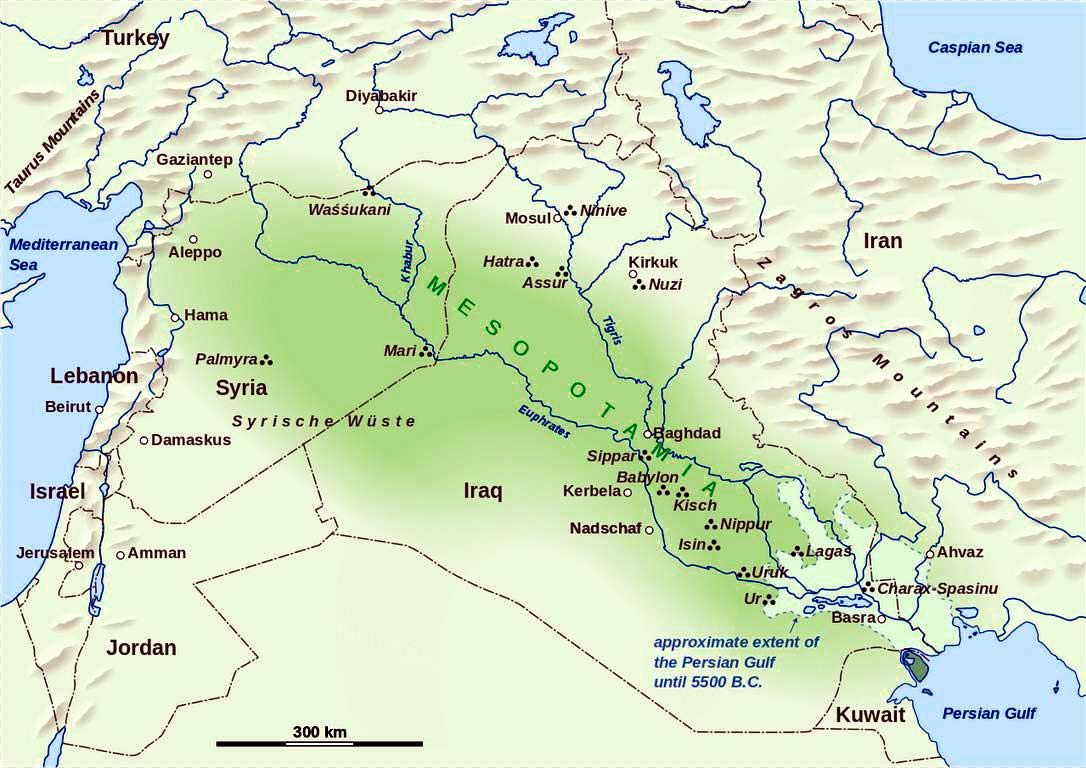
\includegraphics[width=0.8\linewidth]{figure/Map-Mesopotamian-Civilization.jpg}
\caption{Mesopotamian Civilization}
\label{fig:backphoto}
\end{figure}

\begin{figure}[thbp!]
    \centering
    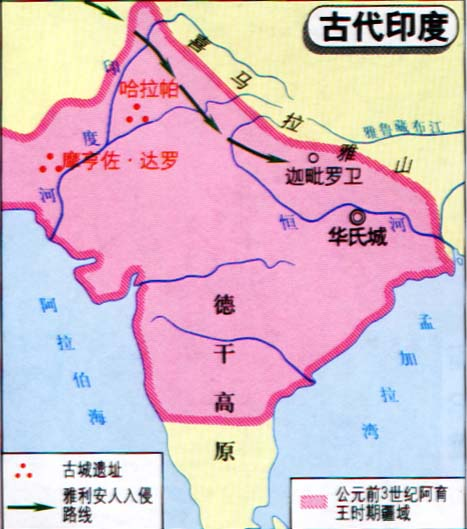
\includegraphics[width=0.8\linewidth]{figure/india.jpg}
    \caption{Mesopotamian Civilization}
    \label{fig:backphoto}
    \end{figure}

公元前3500年以后,苏美尔人在两河流域南部建立起很多奴隶制小国。公园前18世纪,古巴比伦国国王汉谟拉比统一了两河流域,建立起中央集权的奴隶制国家。

地理特点:气候干旱,底格里斯河,幼发拉底河,灌溉农业,处于“肥沃的新月地带”,两河流域不定期泛滥。

苏美尔城邦(神庙为城邦中心),信奉多神教,人与神为从属关系,建筑中最先开始使用拱劵与穹顶。对人类的贡献:发明了楔形文字,成立了培养书吏的学校;发明了车轮(由陶轮而来)。

由于两河流域地势平坦,没有天然屏障,因此常常遭到外族入侵,政权不断更迭。巴比伦时期(古巴比伦王国建立于公元前19世纪,公元前16世纪灭亡)汉谟拉比进行了专制统治(约公元前1792~公元前1750年在位),建立了强大的中央集权国家,并且编制了《汉谟拉比法典》(世界上现存的古代第一部比较完备的成文法典),以维护奴隶主阶级的利益。法典条文共282条,刻在一块巨大石柱上。法典宣扬“君权神授”。它还规定:奴隶可以买卖,还可以用来抵债。如果奴隶胆敢对主人说“你不是我的主人”,他们的耳朵就要被割掉。

国家出现后,美索不达米亚的城市社会中出现了社会等级的分化,导致了负责社会与经济结构的迅速确立,城市中生活着专业劳动者,他们生产出越来越多的高质量产品,又转而刺激了贸易的增长。不仅如此,早期的美索不达米亚还发展出独具特色的文化传统,发明了文字书写系统,组织各种宗教活动。

多产的农业经济推动了世界上最早的复杂社会的发展,大量的人群居住在城市里,在这片广大的区域里扩展他们的政治,社会,经济和文化影响。最古老的城市社会出现在公元前4千年早期的西南亚,尤其是美索不达米亚。
% 为什么出现在这,而不是其他地方
随着人口聚集在城市,需要找到解决争端的办法。争端有时存在于居住地的居民内部,有时事关整个居住地本身,这不可避免地会增加人与人或是团体之间地历史冲突。在寻找秩序地过程中,定居地农业人口承认了政治权威并在整个美索不达米亚建立了国家。国家地出现进一步促进了帝国的建立,某些国家为了扩展他们的势力,加强了自我保护能力,还将周边地区纳入自己的统治。


\subsection{腓尼基文明与希伯来文明}
腓尼基是一系列古代地中海东岸的城邦的总称,是一个海上民族。贡献:商业精神与拼音字母。腓尼基在闪米特语中为“紫色之国”,盛产紫色染料。拼音字母后被希腊学习,成为希腊字母。

希伯来文明的主要支柱是犹太教,希伯来人生活即圣经·旧约内容。

犹太教特点:
\begin{enumerate}
    \item 一神论;
    \item 反对偶像崇拜;
    \item 上帝的选民的思想;
    \item 救世主信仰“弥赛亚”;
\end{enumerate}

\subsection{古代埃及}
"Gift of the Nile" ——古希腊历史学家希罗多德

公元前15世纪,埃及国力强盛,对外征服频繁,疆土不断扩张,成为地跨亚非的大帝国。200多年以后,帝国由盛转衰。公元前6世纪,埃及被西亚的波斯灭亡。

非洲东北部,茫茫沙漠之中,尼罗河蜿蜒北流,每年定期泛滥。水退后留下肥沃的黑土,便于农业种植。约从公元前3500年开始,河流两岸陆续出现几十个奴隶制小国。约从公元前3000年,初步统一的古代埃及国家建立起来。国王自称是神的化身,他们的陵墓金字塔式权利的象征。7世纪,它成为阿拉伯帝国的一部分,古代埃及人逐渐同阿拉伯人融合。

地理特点:
\begin{enumerate}
    \item 位置相对孤立;
    \item 干旱的气候与特定的水源;
    \item 上埃及与下埃及,以孟菲斯未界;
    \item 尼罗河:水利社会;封闭,很少有外族入侵,政治格局变动不大,为大一统的中央集权国家;
    \item 贡献:象形文字,纸莎草;
\end{enumerate}

\subsection{古代印度}

约公元前2500年,印度河流域开始出现奴隶制小国,印度河流域文明兴盛于公元前2500~1700年。

古代印度是一个地理概念,指南亚次大陆,包括今天的印度,巴基斯坦,尼泊尔,孟加拉等国。

地理特点:

\begin{enumerate}
    \item 位于喜马拉雅山南侧统称为印度(为一个地区而非一个国家);
    \item 东,西,南三面环海(东面孟加拉湾,西面阿拉伯海);
\end{enumerate}

公元前14世纪雅利安人进入印度(来自中亚,自称雅利安人。白色人种,身材高大)。征服当地居民并把他们变成奴隶,先后在印度河和恒河流域建立起奴隶制国家,如图\ref{fig:india}所示。

文化特点:“种姓制度”(由雅利安人创造);种姓原意是“颜色”,因雅利安人自视高贵,与当地原住居民区分开。

特点:

\begin{enumerate}
    \item 基于“血统”的等级制度;
    \item 层次(前三等级为雅利安种姓,前二等级为统治阶级,分别对应嘴,手,腿,脚)
    \begin{enumerate}
        \item 婆罗门——祭司阶层;
        \item 刹帝利——国王,贵族武士;
        \item 吠舍——自由民;
        \item 首陀罗——被征服的土著居民
    \end{enumerate}
\end{enumerate}

因而产生规则:种族职业世袭(维护了封建社会长期的稳定性);种族内婚制;排斥外人(由不同阶层混生,不入四个等级);

积极影响:种族制度仍然存在,保证了在外邦入侵和朝代更迭时社会的稳定性。

消极影响:种族制度激化了当时的社会矛盾,并对后来的印度社会的发展带来了不良影响。



\section{古代希腊}

\subsection{爱琴海文明}
公元前2000年左右,希腊早期文明——爱琴文明发祥于克里特岛,后来文明中心又转移到希腊半岛,出现迈锡尼文明。克里特文明和迈锡尼文明合称为爱琴文明。爱琴文明历时约800年后消亡。克里特岛是地中海最大的岛,海岸线曲折,东临爱琴海。

早——爱琴海文明:集中于克里特岛和东大陆伯罗奔尼撒半岛的迈锡尼;

晚——克里特文明:特点:1.中央集权;2.浓厚的宗教色彩;

\subsection{希腊文明的兴起}
希腊文化——荷马史诗:《伊利亚特》+《奥德赛》

\subsection{希腊城邦的建立}
\subsubsection{希腊城邦形成时期}
时间:(公元前8世纪~6世纪)

社会经济文化的进步:出现两百多个小国,史称“城邦”或“城市国家”。城邦面积狭小,人口不多,一般以城市为单位,包括周边若干村落。小国寡民和独立自主构成了城邦的基本特点;

铁器的普遍使用:青铜到铁(铁器的使用提高了生产力,开拓山峦,伐树造船,产生了剩余人口);

海外殖民(在地中海沿岸,围绕爱琴海),与母邦没有从属关系,在经济上联系密切。

文字重新出现(吸收了腓尼基文字的特点,同时首开从左往右写)。

\subsubsection{希腊城邦建立时期}
特点:以城邦为中心,连带周围农村地区(一城一邦,原意“堡垒”,城市与乡村的组合);

希腊早期(公元前8~6世纪)特点:小国寡民(最大8000多平方公里,几十万人口)。

标志城市:斯巴达与雅典。

\textbf{斯巴达(位于伯罗奔尼撒半岛南部)}

特点:并没有沿着雅典城市特有的民主政治发展,而是走向了寡头专制的政治体制,公民生活呈军事化;以农业立国,很少向外移民,而是以征服,扩张的形式,使得国家拥有了大量奴隶,奴隶和土地同属于国家,奴隶人口众多,约十倍于公民人口,因此斯巴达采取了军事化管理,强化自身的军事力量。

表现:1.优生;2.军事化的公民生活;3.“斯巴达式的教育”;4.妇女地位自由,重视妇女教育;

\textbf{雅典(建国,传说忒休斯建国)}

\begin{enumerate}
    \item 忒休斯改革
    
特点:雅典早期贵族统治(贫富分化严重,无力偿还债务者,变为奴隶);
    \item 梭伦改革

目的:为了全社会的利益(梭伦:古希腊七贤之一)

内容:颁布“解负令”(取消债务奴隶,解除了对于公民的威胁,扩大了公民的基础),不以出身而已财产等级,打破了贵族依靠门第垄断政权的局面,而非贵族出身的工商业者,奴隶主提供了参政,仪政的权利;

根据财产多寡,把公民分为四个等级,财产越多者等级越高,权力越大;恢复公民大会(雅典最高权力机构),设立400人会议(分为4个部落,每个部落100人,前三等级均可入选),打破了贵族垄断;

经济改革:设立新的,更受欢迎的陪审法庭来削弱贵族最高法院的权利;每个部落各选一将军组成十将军委员会;

意义:民主政治初现端倪,动摇了旧氏族的贵族特权,保证了公民的民主权利,为雅典民主政治奠定了基础。

    \item 克里斯特尼改革  
    
时间:公元前508年

内容:设立十个区域性部落组织,取代传统的四个血缘部落(按地区划分而不是基于氏族血缘关系,大大削弱了贵族的政治权利);

设立500人会议,由各部落轮流执政,吸收全体公民参政议政(没有财产限制,更加民主)。作用:为公民会议准备议案,同时具有最高执政权和行政权;

“陶片放逐法”作为民主政治的保障;

意义:到公元前500年,雅典已经出现民主政治,雅典民主政治进入成熟阶段。基本铲除了旧氏族的政治特权,公民参政权空前扩大,雅典民主政治确立起来。

\end{enumerate}

\subsection{城邦民主制的建立}

时间:公元前5~4世纪

背景:历时半世纪的希波战争(在亚洲西部波斯帝国不断扩展,侵犯到小亚细亚地区的城邦)

标志战役:
\begin{itemize}
    \item 马拉松战役(公元前490年,地点:马拉松平原),雅典战胜波斯;
    \item 温泉关战役(公元前480年)斯巴达战败,波斯长驱直入;
    \item 萨拉米海战(公元前480年)雅典战胜,波斯返回亚洲;
\end{itemize}

影响:从此世界格局并立发展;希波战争雅典取得盟主地位,民主政治达到全盛;

\textbf{“伯利克里时代”(公元前461~429)}

背景:公元前6世纪,古代伊朗以波斯人为中心形成了波斯帝国,波斯帝国频繁地出征和扩张,先后征服埃及等国际和地区。

公元前5世纪后半期,雅典人口约30万,其中几乎一半是外邦人和奴隶,成年男性公民只有5万。只有六分之一享受“民主”。雅典民主是建立在奴隶制度之上。

\textbf{与现代民主政治的不同}
\begin{enumerate}
    \item 直接民主(而非代议制的间接民主);
    \item 政府官员权利受到限制(任期短,一生只能从事两次);
    \item 全体成年男性公民可以参加最高权利机构公民大会,决定内政,外交,和平,战争等重大问题,他们在行政和司法机构中也发挥着重要作用;
    \item 业余人员组成的政府(有津贴,无专职官员,实行薪给制,贫民有可能担任公职)
\end{enumerate}

缺陷:成年男性公民的民主,无外邦人,妇女,奴隶;

补充:五百人议事会的职能也进一步扩大。陪审法庭成为最高司法与监察机关。法官从各部落30岁以上的男性公民中产生。他们审理各类重要案件,监督公职人员,并参加立法。同时建立许多由陪审团作最后决定的民众法庭,陪审员抽签产生,所有公民都可担任;

为鼓励公民积极参政,向担任公职和参加政治活动的公民发放工资。为吸引公民观赏戏剧,还特意为公民发放“观剧津贴”;

\subsection{古代希腊的文化}

(1) 神话

希腊人的宗教(神与人形象相同,性情也相似)

由此产生了戏剧,古典希腊时代希腊戏剧由政府主持,并且给观剧者发“观剧津贴”;

(2) 建筑

也由希腊宗教传说发展而来,包括雅典帕特农神庙,是为了供奉雅典娜女神而建。

材料由大理石而建,同时神庙的功能,不仅是城邦公民生活和商业活动的场所,而且还储藏着公共财富。

特点:1.方顶柱式结构;2.长方形的神庙殿堂;3.四周高大的圆柱柱廊;

(3) 哲学

希腊三贤:苏格拉底,柏拉图,亚里士多德

苏格拉底:拥护贵族统治,反对当时实行的城邦民主制;

柏拉图:哲学思想“理念论”;政治思想学说;“理想国”,同时在雅典城邦建立学园;

亚里士多德:“百科全书式”的学者

(4) 历史

希罗多德(西方史学之父)——《历史》(描述希波战争,歌颂雅典)

修昔底德《伯罗奔尼撒战争》(描述雅典与斯巴达之战,雅典战败)主张从客观,批判的角度看待历史。

\textbf{总结}

古代希腊是欧洲戏剧的故乡,涌现出许多著名的戏剧家。除索福克勒斯外,还有著名的“悲剧之父”埃斯库罗斯,以及“喜剧之父”阿里斯托芬。埃斯库罗斯的作品大都通过神话题材表现雅典政治制度和伦理道德的斗争,语言雄浑有力,寓意深刻。阿里斯托芬则用喜剧讽刺当时的政治,宗教和伦理道德。

雅典民主的理论与实践,为近现代西方政治制度奠定了最初的基础。民主氛围创造的空间,使雅典在精神文化领域取得辉煌成就。

雅典民主更是小国寡民的产物。过于泛滥的直接民主,成为政治腐败,社会动乱的隐患。选举和轮流执政,不能保证参议员的素质,国家权力有时成为社会不公的一种暴力机器。狭隘的城邦体制,最终无法容纳政治和经济的迅速发展。公元前4世纪后半期,日渐衰微的希腊被北部崛起的马其顿王国所灭。

实质:希腊民主是建立在奴隶制基础上的少数人的民主,维护的奴隶主贵族的利益。

\subsection{亚历山大帝国}

公元前4世纪下半叶起,希腊北部的马其顿崛起。

国王腓力二世改革,于公元前338年征服了希腊城邦,遭遇刺杀后,其子亚历山大大帝继承王位,征服了希腊,并向东扩张,打败了波斯帝国,最后其疆域地跨亚欧非三大陆,如图\ref{fig:亚历山大帝国}所示。

亚历山大帝国开启了人类历史上的新纪元,将东西方文明连接起来,最后定都巴比伦。政治措施:1、入乡随俗;2、联姻政策;3、移民


亚历山大去世后帝国一分为三:1、马其顿王国(希腊部分);2、埃及的托勒密(维持时间最长);3、塞琉西亚王国(以叙利亚为中心);

\subsection{希腊化时代的文化}

亚历山大东征后帝国重心东移,如埃及的亚历山大城。期间科学迅速发展,原因:1、希腊城邦时代的思想基础;2、近东的资料;3、王国政府的支持;

\subsection{古希腊乌托邦思想}

\section{古代罗马}
\subsection{罗马共和国的兴起}
公元前8世纪,在意大利的台河河畔,罗马城逐步建立起来。公元前509年罗马建立了共和国。

罗马共和国的兴起:罗马城源于台伯河河畔的若干部落的联合,即所谓的“七丘同盟”。

罗马早期共和国制度包括:
\begin{itemize}
    \item 执政官:均为贵族担任,正常有两个执政官,当有战事发生时,其中一个可被推选为独裁者;
    \item 元老院:由贵族组成,掌握国家的财政和军事,同时拥有对百人团大会决议的通过权,实际上拥有了国家的最高权力(早期贵族垄断着立法和司法大权,当时罗马只有习惯法,法律与习惯之间没有明显的界限。常常损害平民利益);
    \item 百人团大会:其中元老院贵族终身任职。“法西斯”象征着国家的最高权威。平民与贵族的斗争贯穿于罗马早期共和国历史。
\end{itemize}

(法西斯:古代罗马共和国时期的最高行政长官,有12个卫士相随。他们各手持一束棍棒,束棒中间插有一把战斧,象征着罗马国家的最高权利。棒子用于执行笞刑,斧子用来执行死刑。“束棒”在古代罗马人使用的拉丁语中,读作“法西斯”(fosces)。法西斯主义一词由此发展而来。

现代法西斯专政,是垄断资产阶级对内实行的极端专制的恐怖统治。)

方式:1.从战场上撤离;2.保民官(由平民推选),对贵族元老院的决策行使否决权,保障平民利益;

“十二铜表法”(贵族妥协后落实)。由于这些条纹镌刻在12块铜板上发表,故名。它涉及公法与私法,刑法与民法,同态复仇法,氏族继承与遗嘱等。

意义:是罗马第一部成文法典,传统的习惯法汇编而成,按律量刑,有法可依,对罗马法体系乃至近代欧洲都产生深远影响。

\subsection{罗马的扩张}

背景:经过平民与贵族的不断抗争,最终平民取得了较实质性的保障,国家趋于稳定,国力强盛。

公元前3世纪早期,罗马征服并统一了意大利半岛,然后向地中海地区扩张。公元前27年,罗马帝国建立,至1世纪后期,罗马帝国已经建立了30多个海外行省,控制欧亚非三大洲的广阔疆域,统治了许多不同的民族。

路线:1.先征服了意大利半岛;2.经过了三次“布匿战争”征服了西地中海;3.经过三次马其顿战争征服了东地中海。

主要原因在于罗马拥有优越的军事组织,在继承希腊的军事战略的同时又自我发展,形成了以军团为编制,军纪严格的军队。

对西地中海的征服中,由于罗马人称迦太基人为布匿人,史称布匿战争,持续了一百多年,可以分为三次较大的战争。

在第二次布匿战争(公元前218~201),迦太基(曾是腓尼基人在北非建立的殖民地)中诞生了一位卓越的军事将领汉尼拔,率军侵入意大利,征战15年不败。在最后一场战役中(公元前149年),罗马军队战胜了汉尼拔,迦太基头像(公元前3世纪末打败,迫使迦太基放弃了非洲以外的所有土地,并向罗马交付了大量赔款和几乎全部的舰只)。由于罗马人担心迦太基发展国力后东山再起,于是借机发动第三次布匿战争,彻底征服了迦太基,将其变为自己的一个行省。

经过三次马其顿战争,征服了东地中海。从此罗马彻底统治了地中海地区,将地中海变为自己的“内海”,清除了海盗,大力发展海上贸易,国力强盛。

罗马扩张后果:
\begin{itemize}
    \item 奴隶制的发展:奴隶源源不断地涌来,同时不被视为人看待;
    \item 大土地所有制的发展:服兵役的农民回家后穷困潦倒,不得不将自己的土地卖给贵族,贵族因此大肆兼并小农的土地;小农的破产导致罗马兵源的枯竭,罗马的公民制走向瓦解,而且罗马兵源的枯竭导致罗马共和国后期的冲突不断;
    \item 在征服过程中,不同民族之间的矛盾显现出来,特别是被征服者,由于得不到公民法的保护,对罗马统治表现出强烈不满。随着版图的扩展,国际交往的扩大,商品经济与贸易的发展,在政治经济活动中也产生了许多新问题,新矛盾。显然,仅适用于罗马内部的公民法已无法应对这些新变化;
\end{itemize}

为巩固统治,帝国对行省上层阶级大量授予公民权,对无公民法的外邦人给以适当的司法保障。3世纪,帝国境内自由民内部公民的区别不复存在,万民法成为适用于罗马统治范围内的一切自由民的法律。

\subsection{罗马共和国的危机与衰亡}

公元前1世纪,罗马发生了严重的社会危机。共和制再也无力统治,奴隶主企图建立独裁统治,以稳固政权。由于奴隶与奴隶主的冲突不断,因而奴隶们不断地爆发起义,其中最大的为斯巴达克斯起义(公元前73~71年),苏拉建立军事独裁(公元前49年)后,凯撒登上了历史舞台。

关于凯撒的三点:1.与庞培,克拉苏结成“前三头同盟”;2.远征高卢;3.托勒密王朝,埃及艳后;

在克拉苏死后,与庞培决裂,最后将罗马权利揽于其身,建立了独裁统治,结束了贵族的共和统治。贵族由于自身权利受到侵犯,于是刺杀了凯撒。之后其子屋大维崛起(公元前63~14年),与安东尼,李必达结成“后三头”同盟。并崛起后各自划分军政范围。屋大维在公元前27年开始独揽国家大权。屋大维最终与安东尼决裂,屋大维在打败安东尼后征服了埃及,托勒密王朝结束。

\subsection{罗马帝国的建立}

罗马帝制的建立(由屋大维建立,避开“独裁者”的身份,支持元老院的存在,但已名存实亡)。

“第一公民”,“首席元老”或“元首”;“奥古斯都”(拉丁文意为至尊或神圣);罗马帝制正式创立(屋大维成为第一位皇帝);“元首政治”是一种隐蔽的君主制(屋大维表面上维持共和国的框架,尽量尊重元老院地位)

屋大维为稳定帝国采取的措施:
\begin{enumerate}
    \item 改组军队,忠于自己;
    \item 消除社会动乱因素,通过“面包和竞技场”(来稳定社会上的无业游民);
    \item 推进罗马城市建设;
    \item 争取意大利同盟者的支持;
    \item 缓和对行省的政策(取消以前对各个行省的剥削)
\end{enumerate}

屋大维死后,立每年的8月为“奥古斯都日”,“August”

罗马摆脱了共和国晚期的动乱局面,经历了三个典型王朝(公元前14~公元前180年)。罗马帝国在最初的大约200年里,呈现出繁荣景象,是当时最强大的帝国之一。

屋大维统治罗马后,罗马多次发动侵略战争,帝国疆域不断扩大。到2世纪,它的疆域达到最大规模,东起幼发拉底河上游,西临大西洋,南抵非洲撒哈拉大沙漠,北达不列颠,莱茵河和多瑙河。

各个王朝

\begin{enumerate}
    \item 朱里亚·克劳狄王朝(公元前27年-公元68年)
    
尼禄是西方历史上一位著名的暴君,加剧了各个行省的矛盾冲突。 

\item 弗拉维王朝(69年-96年)

镇压犹太人起义,派重兵镇压耶路撒冷的犹太人起义。“犹太人”离散时期。

\item 五贤帝统治时期(公元前96~180年)

通过过继制度继承王位,是中央政权最稳定时期,即“黄金时代”。
    
\end{enumerate}

\subsection{基督教的产生及其早期发展}

\subsubsection{基督教的产生}
产生:公元1世纪20~30年代

基督教于1世纪诞生。起初,基督教信徒组成许多小宗教团体,后来这些小团体逐渐形成统一的基督教会。4世纪,罗马皇帝确定基督教为国教,大大促进了基督教的传播。后来,基督教逐渐传遍全欧。11世纪,基督教分裂为天主教和东正教,分别以罗马和君士坦丁堡为中心。

基本观点从犹太教中诞生,进而发展为普世宗教。

圣保罗对基督教的贡献:1.耶稣就是救世主;2.将基督教变为一种普世宗教。

《圣经》包含《旧约》和《新约》,《旧约》指上帝通过摩西与犹太教所定之约,而《新约》指上帝通过耶稣与信者另立之约。早期基督教徒受罗马当局迫害。

\subsubsection{基督教的发展}

基督教合法化的相关背景:
\begin{enumerate}
    \item 传播范围的扩大,信众人数增加,社会势力上升;
    \item 社会构成的变化
    \item 教义的变化:从主张平等,博爱,财产共有,互助合作到倡导劝人驯服,爱仇如己,忍受现实苦难,即从反抗的倾向转变为容忍的色彩。
\end{enumerate}

\subsubsection{基督教合法化}

过程:公元313年君士坦丁堡一世颁布“宽容赦令”——米兰赦令,承认基督教的合法地位。公元392年,皇帝狄奥多西一世正式宣布基督教为罗马的国教。至此,基督教才与帝国的政权相结合。

\subsection{罗马帝国的衰亡}

罗马帝国的成就(总人口达7000万以上)

维持了广大地区的秩序和稳定;普及公民权于各个行省,基本消除了征服者于被征服者的矛盾;建立了罗马共同体;建立了罗马公路网,交通四通八达;海上贸易繁荣 

原因:五贤帝时期最后一位皇帝没有将过继延续,最后酿成了罗马帝国时期“三世纪的危机”。

公元235~285最动荡时期:政局动荡和离心的倾向,和对王位的争夺,以及蛮族的威胁,日耳曼人的入侵,内部奴隶起义,基本造成了罗马帝国的崩溃,但由于公元3世纪末和4世纪初戴克里先和君士坦丁改革,维持了一段稳定。

主要内容:
\begin{enumerate}
    \item 公开的帝制——公开宣布君主制;
    \item 干预经济生活(将一定数量的土地和农民捆绑起来);
    \item 把帝国分为东西两部分,分别两位君主统治(395年);
    \item 加强宗教;
\end{enumerate}

君士坦丁则建立起东罗马帝国的新首都君士坦丁堡,在短期内加强了帝国统治,使罗马帝国度过了世纪危机。但于公元4~5世纪,罗马帝国崩溃。

蛮族入侵:

日耳曼人进入罗马帝国境内(由于受匈奴人西进驱赶);410年,日耳曼人分支之一西哥特人首次攻陷罗马;455年,汪达尔人再次攻陷罗马;476年,西罗马帝国灭亡(西欧封建社会的历史随之终结,东罗马帝国继续存在到15世纪中期)

\subsection{古代罗马的文化}

\subsubsection{宗教与文化}

罗马文化初期注重对希腊文化的传承,并且在希腊文化中融入了他们务实的风格。

宗教:古代罗马发展起的多神崇拜,深受希腊影响;

主神:朱庇特——宙斯;天后:朱诺——赫拉;智慧女神米涅瓦——雅典娜;战神:马尔斯——阿瑞斯;大力神:赫丘利斯——赫拉克里斯;美神:维也纳——阿芙罗狄黛;商旅之神:墨丘利——赫尔梅斯;胜利女神:维多利亚——尼凯

金星:维纳斯;木星:朱庇特;水星:墨丘利;火星:马尔斯;土星:萨图恩(农神)

希腊宗教特点:展示人性(人与神同性同形),而罗马的宗教则主要为政治性。

\subsubsection{语言与文字}

罗马使用拉丁字母,为以后欧洲各天主教文字作铺垫。

文学:维吉尔的史诗,贺拉斯的田园诗,奥维德的情诗。

建筑:古代罗马建筑,继承了希腊的建筑成就,包括穹顶,拱券。其建筑之所以更辉煌,在于将火山灰投入建筑使用中,加上沙,石头,基本等同于混凝土,方便按模具灌注成型。
\section{西欧封建社会的形成与发展}
\subsection{前言}
从476年西罗马帝国灭亡,到1500年左右的欧洲历史,被西方史学家称为“中世纪”。它是古代希腊罗马文明消亡与近代资本主义社会产生之间的一段历史。中国史学家习惯上称之为西欧封建社会。

\subsubsection{西欧主要封建国家形成与发展}

西罗马帝国灭亡后,日耳曼人在其领土上建立起几个国家。其中的法兰克王国,发展为西欧的一个大国。在查理统治时期,法兰克王国达到全盛。800年,建立了查理曼帝国。814年,查理去世,他的子孙庸碌无能,相互倾轧,国家陷入混乱。843年,他们将帝国一分为三。后来,从这三部分,分别发展为法兰西,德意志和意大利三个封建国家。5世纪中期,在日耳曼人迁徙浪潮中,他们当中的盎格鲁,撒克逊等部落从欧洲大陆进入不列颠,建立了一些小的国家。这些国家长期兼并,9世纪,开始形成早期的英吉利王国。

但是,在这些秀国家中,政治的发展曲折艰难,国家长期四分五裂,统一的中央集权国家很晚才出现。直到15世纪,英国和法国菜通过强化王权,剪除大封建主实力的措施,建立起统一的中央集权国家。德意志的情况更加糟糕。从查理曼帝国分裂出来的东法兰西,逐渐发展为德意志国家。德意志国王奥托一世,野心勃勃,大举向意大利扩张,在教皇的支持下,在10世纪建立起所谓的“神圣罗马帝国”。然而,由于皇帝权利受教皇和封建主的掣肘,帝国徒有虚名。此后的几百年间,帝国内的诸侯势力强大,根本不把皇帝放在眼里。到14世纪时,帝国境内还存在七个诸侯国,处于诸侯割据的状态。在很长的历史时间里,德意志境内关卡林立,交通不便,封建混战频繁。直到19世纪中期,德意志仍存在几十个小邦,处于四分五裂的状态,统一的中央集权国家迟迟建立不起来。19世纪六七十年代,其中最强大的普鲁士才统一了德国,建立了封建性很强的军事专制统治。意大利的情况与德意志基本相当,长期处于封建分裂状态中。

西欧封建社会时期,教皇与教会不仅是西欧最大的土地所有者,还是西欧封建制度的精神支柱。他们加紧对人民的精神统治,残酷压制与教会观点相悖的“异端”思想。在精神和文明领域,神权凌驾于一切。当时的百姓多是文盲,教会完全垄断了对基督教经典《圣经》的解释权。任何背离教会的说教和反对罗马教廷教义的思想都被当做“异端”。13世纪,教会建立起“宗教裁判所”,对“罪名”成立的“异端”分子实行判决,轻者罚款,重者监禁,有的甚至被捆在火刑柱上烧死。

\subsubsection{西欧封建社会的政治——体系严密的封建制度}
西欧封建社会早期,土地是主要财富。国王把一部分土地分封给分封给大封建主,这些人成为诸侯,诸侯又把一部分土地分封给较小的封建主,小的封建主再向下分封。国王和大封建主又各自分封了一批骑士,作为自己的武装力量。

这样层层分封,就形成了各种自大到小不同等级的封建主。这些封建主分别领有大小不等的封地,拥有数量不等的庄园,农奴和武装。这样,在社会的每个角落,形成一种领主(封主)和附庸(封臣)的关系,他们彼此负有义务。领主保护附庸,附庸必须向领主宣誓效用,为领主提供多种服务,包括:发生战争时军事上要援助领主;领主到访时根据礼仪进行接待;领主的女儿结婚时送礼致贺。但是,领主只能管辖自己的附庸,不能管辖附庸的附庸。每一个封建主无异于一个小的国军,割据一方,各自为政。诸侯的势力很大,有的竟敢向国王挑战。封建贵族住在戒备森严的城堡里,有自己的武装;他们的经济单位叫庄园,一般自给自足,不与外界交往。结果,严格的封建等级制度,辽阔庄园环绕的无数城堡以及直插天际的尖顶教堂,成为西欧封建社会早期的典型政治风貌和独特的社会景观。

\subsubsection{政教冲突}
从5~6世纪始,西欧的教诲势力迅速增长。罗马天主教会是最有势力的封建领主,他拥有天主教世界土地的三分之一。教诲同样按照封建的方式建立起自己的教阶制度,最高的是教皇,下面是大主教,主教等,他们各有自己的辖区。

8世纪中期,意大利中部出现教皇国。教皇既是宗教领袖,同时又是拥有世俗权力的一国之君,直接管辖的领土达四万多平方千米。国王为了使自己的统治神圣化,经常请求教皇以上帝的名义为自己加冕。查理大帝就是这样做的。这种做法加强了封建国王与教会的联系,更意为着教权凌驾于王权之上。9世纪,教皇成为西方基督教世界中的仲裁者。然而,教皇与封建君主时而相互勾结,时而明争暗斗。12~13世纪,经过长期的争斗,教皇权利达到了顶峰,教皇有权废黜君主;罗马教廷成为中欧和西欧一切宗教事务和教义问题的最高总裁机构。只是到了中世纪后期,随着西欧中央集权国家的形成与壮大,资产阶级的兴起,文艺复兴,启蒙运动和宗教改革的发展,教皇和罗马天主教会的势力才逐渐衰落下去。

\subsubsection{城市的兴起}
11~12世纪,欧洲各地的城市普遍重新兴起。中世纪时,由于人口的增加和商业的发展,除原来罗马帝国时期的老城市外,在城堡,主教堂,大修道院附近地区出现了许多新兴城镇。法国的巴黎和马赛,英国的伦敦,德意志的科隆等都是当时的著名城市。14世纪时,伦敦人口有4万,巴黎有8万。西欧城市工商业和手工业发达。随着技术的不断发展,手工业的行业分工日益精密。同一行业的人们组成行会,行会雨后春笋般地出现。

在西欧城市重新兴起和工商业迅速发展的过程中,市民阶级形成了,并从中进一步分化出手工业者,商人和银行家等等。商人和银行家成为市民阶级的上层,发展为早期的资产阶级。广大西欧城市开展了争取自治权利的斗争,并制定了自己的法律,建立了自己的武装,向封建王权和各封建主发起了挑战。一些城市里,如法国的巴黎,英国的牛津和剑桥等还建立了大学,成为著名的大学城。到14~15世纪,从西欧封建社会内部发展起来的新兴的城市中等阶级,以及与封建制度水火不容,成为西欧反封建王权的强大革命力量。

\subsubsection{封建等级代表制的出现}
13世纪早期,欧洲一些王国的君主竭力重振王权,将地方权力收归中央。英国国王约翰横征暴敛,没收教会田产,引起了贵族和教会领袖的不满。强大的封建贵族联合教士,小封建主和市民举行武装反抗。经过斗争,约翰被迫承认教会选举自由;不向封建主征收额外的捐税;承认伦敦等城市已享有的自由。结果,王权收到封建法律的约束,国王的独断专行收到限制。国王不甘心权利的削弱,挑起内战,国王战败。13世纪后半期,英国的议会制度开始萌芽,以后议会逐渐开始定型为上下两院。国王必须通过议会规定赋税,制定法律。等级代表制的封建君主政体对国王权利有所制约。14世纪初,法国也出现了以三级为代表的等级代表制,由于法国王权比较强大,三级会议限制王权的作用相对较小。

英国的等级代表制度对西方政治制度的发展影响巨大,在反对封建国王专制集权的斗争中,封建贵族,高级教士,城市商人等联合起来斗争,迫使国王坐下来,与他们商讨有关征税等关系国计民生的重大问题,使封建王权收到制约。英国的等级代表制在制约王权,建立资本主义制度的斗争中起到了重要作用,成为西方近代议会制度的起源。


\subsection{日耳曼人的入侵及其影响}
公元5世纪末,西罗马帝国灭亡,一系列日耳曼帝国崛起,西欧开始步入封建社会,这个时期的西欧经济以封建庄园制为主,政治上长期处于王权羸弱分裂割据状态。

日耳曼人为游牧部落,于公元3-5世纪,在匈奴人的驱赶下进入西罗马帝国并逐步进行了征服。同时日耳曼人属于蛮族部落,具有两个特点:1.原始社会末期的氏族部落;2.军事民主制阶段;

日耳曼人入侵的后果:

1.改绘了当时西欧的政治地图,重组了民族格局;

2.造成了巨大的社会经济破坏(由于日耳曼人文化经济水平落后,无法继承罗马的文化);

罗马的封建制因素和日耳曼人的氏族制因素结合并最终导致了西欧封建社会的形成。

日耳曼人的特点:

\begin{itemize}
    \item 没有国家观点和行政管理机构;
    \item 法律简单,神裁法;
    \item 自然经济;
    \item 日耳曼征服者在各方面不同程度上受到了罗马文化的影响;
    \item 皈依罗马天主教,反映了当时蛮族罗马化的趋向;
\end{itemize}

\subsection{法兰克王国}
日耳曼人创立的王国中存在时间最长的。后来,在法兰克王国的基础上,建立起意大利,法兰西和德意志。

\subsubsection{墨洛温王朝(481-751)}
在496年统治者克洛维正式皈依了基督教罗马教会,这种政治需要开启了日耳曼人与罗马人结合的起点(王权与政权结合)。

之后其子统治时期庸碌无能,由宫相掌管国家大事。8世纪前期,查理·马特成为宫相,进行采邑制改革,改变以前无条件赏赐贵族土地的做法,实行有条件的土地分封,得到封地的人必须为封主服兵役。其意义在于将土地以采邑的形式分封给参战的战士,条件是为中央政权服兵役。这就在封主和封臣之间建立起了明确的权利和义务关系。9世纪后期,这种封地逐渐变成了世袭领地。后来,国王以下的封建主也把土地当做采邑分封出去。逐层分封的结果,形成了不同等级的封建主:公爵、侯爵、伯爵、子爵、男爵、骑士。这封建等级制度中,每个人对其上级来说都是附庸,对其下级来说则是封建主,各级封建主依次从属,每个封建主只能管辖自己的附庸,而无权管辖自己附庸的附庸。

大封建主居住在讲究城堡里。城堡既是住宅,有是防卫措施,周围筑起高墙,墙外挖有宽阔的壕沟。城堡内备有武器,存放着充足的粮食和生活用品。

影响:1.变更了土地占有关系,促进了以土地为纽带的封建等级制的形成;2.在封建贵族内部形成了严格的等级制度。

\subsubsection{加洛林王朝(751-843)}
751年其子丕平即位,由于丕平不满宫相这一地位,为篡夺王位,与基督教会勾结。篡位成功后,为表感恩之情,两次进攻与教皇作对的人,把罗马到拉凡纳的一片土地奉献给教皇,史称“丕平献土”。教皇以上帝的名义为他加冕,这种做法加强了国王与教会的联系,使教权凌驾于王权之上,而且教皇辖地的疆域从此得到了奠定。在意大利中部出现了教皇国。十二三世纪时,教皇国势力鼎盛一时,754年得到罗马皇帝的加冕。

西欧封建社会时期,罗马教廷有至高无上的权利。在西欧长期动乱的过程中,基督教会乘机扩大势力与影响。法兰克等国君主接受了基督教,并向教会大量赐赠地产。教会本身也巧取豪夺,占有大量土地。

\subsubsection{查理曼帝国}
法兰克达到全盛时期,在此期间教廷与皇权达到空前的结合。查理大帝支持罗马教廷。

800年,教皇为查理加冕为“罗马人的皇帝”,至此,日耳曼人完成与罗马的结合。公元843年《凡尔登条约》,查理曼帝国一分为三。


\subsection{封建制度与封建庄园经济}
在法兰克帝国时期,由于王朝混乱,各领主自己招募士兵,成为当地的保护着。

\subsubsection{封建制度}
源自拉丁语“封土”,即封军赋予义务的土地,有条件地占有土地;封建制度是以土地占有权和人身关系为基础的社会制度,在这种关系中封臣从封君得到一块土地,同时向封君履行一定的义务。

两大源头:日耳曼因素,罗马因素。

\subsubsection{封臣制度}
采邑,终身占有,不是世袭;查理·马特军事改革,采邑制度普及。重装骑兵,全身盔甲;

世袭采邑;统治权(司法权)与土地所有权的结合,即领主封臣制与大土地产馈赠的结合。

西欧封建制度核心(封君封臣关系)

封建法规:规范封君与封臣关系,相互的权利与义务关系;

骑士精神:忠勇,仗义,尊重妇女,保卫基督教;(参考《唐吉坷德》)

\subsubsection{庄园制度}
地位:1.封建庄园是整个西欧封建时代农村基本的经济与社会组织;2.国王,贵族和教会都是庄园的领主。

特点:1.经济上自给自足,除盐铁外,所有都可以在庄园里自己完成;2.社会生活上自给自足(教堂,教士);3.农奴没有人身自由,农奴的义务:服劳役,捐税和使用权;4.领主有责任保护农奴;

庄园分为三部分:领主的自营地,农奴的分地和自有佃农的分地。

封建庄园经济是一种经济上自给自足,政治和宗教上大体独立的社会实体。(参考英剧《唐顿庄园》)

\subsection{西欧经济的复兴}
经历过“黑暗的中世纪”之后,西欧经济逐渐走向复兴。

\subsubsection{农业革命}
使用了中世纪的重犁,可以开发西欧湿重的黏土,增加了作物的种植面积;

谷物轮种的三田制,替代了原先的二田制,即分为冬季作物,春季作物和休耕三部分,从而每年能收获三分之二;

风磨和水磨的发明,使得劳动率提高,耕种面积扩大,农产品产量显著增加,出现了剩余。也是中世纪城市兴起于发展的基础。

\subsubsection{贸易复兴}
两大贸易区:

南部以意大利的威尼斯,热那亚和比萨等城市为主的地中海贸易区;北部贸易区以佛兰德尔的布鲁日等城市为中心的北海贸易区;

定期市集,最著名的香槟市集(长途搬运货物的交易集所)。

\subsection{中世纪城市的兴起}

\subsubsection{工商业城市的起源}
城市多兴起于交通便利,相对安全,容易获得廉价原料和销售产品的地方。海湾地区,如意大利的威尼斯;港口附近,如英国的牛津;堡垒附近,如英国的曼彻斯特。

当时的城市规模不大,一般围有城墙和供守望用的城堡。除教堂和市政厅等较大建筑外,房屋低矮,街道狭隘,拥挤,纵横交错。沿街商店,住房和作坊鳞次栉比。有些手工业者兼营农牧业,街上牛,羊,猪,鸡,鸭等随处可见。白天嘈杂喧嚣,夜晚万籁俱寂。

随着城市的发展,阶级冲突日益尖锐。西欧城市是在教会或世俗封建主的领地上产生的。随着商品经济的发展,封建主日益贪婪,对城市市民加紧剥削。

三个主要途径

\begin{itemize}
    \item 罗马古城遗址上建立新城;
    \item 军事城堡(可以保护手工业者和商人从事交易,因而逐步发展为城市);
    \item 商业中心,如威尼斯;
\end{itemize}

以上城市往往在封建领地里发展起来。10世纪开始出现作为手工业和商业中心的城市。意大利,法国,英国,德意志等都有许多著名城市。

城市可以分为:a.城市国家;b.自治城市;c.自有城市;

根据自治程度的不同来划分,部分工商业城市还具有国家职能,如征战。同时获得自治的途径有多种,如赎买,武装斗争等。

\subsubsection{城市兴起的意义}

1.促进了欧洲工商业的发展和乡村经济的商品化(如乡村原有的实物地租变为货物地租);

2.导致了农奴制的瓦解(在城邦居住可获得自由民的身份,免除债权和义务);

3.孕育了新的社会阶层——城市中产阶级(原先中世纪等级有三:教士,贵族,农民);

\subsection{十字军东征}
时间:1096-1270年

11世纪末起,在罗马教廷的倡导下,西欧教俗封建主及大商人组成联军,以向进犯“圣地”的伊斯兰教徒展开“圣战”的名义,对地中海东部地区发动了持续近200年的侵略性的军事远征。

各个阶层参加东征的原因:

\begin{itemize}
    \item 教会:收复“圣地”;
    \item 封建领主和骑士:夺取土地和财富;
    \item 普通基督教徒:宗教信仰,教会许诺的利益;
    \item 商人:扩大商业利益;
    \item 农民:摆脱困境,获得自由。从穆斯林手中夺取“耶路撒冷”,即所谓的宗教热情。
\end{itemize}

导火索:1095年,罗马教皇召开克勒芒宗教会议,号召拯救圣城。

十字军东征的过程(1086-1270)

\begin{itemize}
    \item 第1,2,3次东征的目标是耶路撒冷及其周边地区;
    \item 第4次东征的目标是拜占庭帝国;
    \item 第5,6,7次东征的目标是埃及;
    \item 第8次东征的目标是北非的突尼斯
\end{itemize}

第一次东征时攻陷了耶路撒冷,并且进行了大屠杀。之后建立的十字军国家(1.埃德萨伯国;2.安条克公国;3.耶路撒冷王国;4.特里波利波国)

第三次(1189-1192),第四次(1202-1204)教皇英诺森二世率军攻下了拜占庭首都君士坦丁堡。

东征的后果和影响:

1.侵略战争的性质;

2.消极影响:使东方的物质文明遭到了破坏,阻碍了其社会经济的发展;

3.积极影响:客观上以野蛮的方式促进了东西方文明的交流与传播;

4.教会势力的消长;

\subsection{中世纪的法国}
中世纪的法国是西欧最早形成的民族国家。法国中央集权的加强,由法王腓力二世执政(1180-1223)。利用联姻,作战等方式,从英国统治区域收复了大量失地。

腓力四世与罗马教廷的斗争以王权胜利告终,罗马教廷也迁都到阿维农,史称“阿维农之囚”,操纵教廷长达70年。

腓力四世在于罗马教廷的斗争中为争取民众支持,召开会议(三级会议)。1302年,在巴黎圣母院召开了第一次三级会议,三个等级分别是:教会上层人士,世俗贵族和市民上层代表。会议标志着法国等级君主制形成,各个封建等级分享政权。路易十四时达到绝对君主制的顶峰。

\subsection{中世纪的英国}
在中世纪时期英国的权利很大。起于1066年的诺曼征服。威廉成为国王,加快了封建化进程。威廉一世为加强王权,采取措施如下:

\begin{enumerate}
    \item 将土地作为战利品分封,威廉实际上成为了英格兰最高土地的所有者;
    \item 进行土地大清查,制订了《土地赋役调查薄》,作为国王征收赋税的依据;
    \item 保留了盎格鲁-撒克逊人的郡制,设置了郡长和郡法庭。威廉要求土地所有者先向国王效忠,再向领主效忠,加强了王权;
\end{enumerate}
	
中世纪的英国设立了普通法,基本内容是司法判决案例,受到传统习俗,罗马法和宗教法的影响,又自成体系。在盎格鲁-撒克逊人的习惯法基础上,把全国各地的习惯法集中起来。扩大了法庭的司法权限。

\subsubsection{《大宪章》的签订与议会的召开}
1215年“失地王”约翰被迫签署《大宪章》

主要内容:限制王权,保障贵族,骑士和市民的权益;

《大宪章》以法律约束王权,王位与法律,对维护封建秩序有积极作用;保障市民的商业权利,有利于城市经济的发展;促进了英国议会;

开端:
\begin{enumerate}
    \item 1265年召开贵族,骑士和市民代表参加的全国性大会;
    \item 1295年议会被称为“模范议会”,标志着英国等级君主制的形成(由贵族议会到等级议会);
\end{enumerate}

\subsubsection{英国议会政治的发展}
最初为监督《自由大宪章》和保障贵族,骑士和市民权益的政治机构,后权限逐渐扩大。1297年获得批准征税的权力。14世纪初获得颁布法律和审理政治案件的权力。1343年,议会形成两院制,其中上院由贵族代表组成,下院由骑士和贵族代表组成。

\subsection{中世纪的西欧文化}

\subsubsection{中世纪的教育}
中世纪开始兴办大学,大多由神院发展而成。“大学”意为“总和”“联合”,即由学生和教师组成的行会。“院系”意为“才能”。中世纪大学不隶属教会,不依附地方,由学费经营。现在的学位制度源自中世纪欧洲。1500年全欧80所大学。

文学主要以拉丁文学和方言文学为主。特点是浓厚的宗教色彩。早期以拉丁语来创作。在11~13世纪,方言文学兴起,以英雄史诗,骑士抒情诗和骑士传奇与寓言为主。如法国的《罗兰之歌》,德意志的《尼贝龙根之歌》,英国的《亚瑟王传奇》。

\subsubsection{中世纪的建筑}
主要建筑风格为罗马式和哥特式。11世纪时,西欧经济发展,封建经济稳固,作为社会精神支柱的教会势力发展很快,不断兴建教堂和修道院。为了追求壮观的效果,这些建筑普遍采用类似古罗马建筑中拱顶与梁柱的结合,这中新的建筑样式被称为罗马式建筑。罗马式建筑多使用石头屋顶和圆拱,并用复杂的骨架结构来建筑拱顶。教堂平面设计的十字架形,是罗马式建筑的主要特点。罗马式教堂的外形像封建领主的城堡,窗户很小,而且距地面较高。

12到15世纪,欧洲盛行哥特式建筑风格。意大利学者认为,这一时期的建筑缺乏艺术趣味,所以用“蛮族”哥特人一词,称之为哥特式、哥特式建筑由罗马式建筑发展而来,但已不是城堡的样式。它的造型风格以高,直,尖和强烈的向上感为特征。哥特式建筑结构轻盈,纤细,大量使用小尖塔,并装有五颜六色的彩色玻璃。罗马式出现在早期9-12世纪,其中穹顶,后壁,窄窗,圆柱为主要特色。光线黯淡,给人以神秘感,渗透以罗马理性,实用的生活态度。哥特式出现在12-15世纪,高,直,尖,体现对天国的向往。薄墙壁,大窗户,高耸的尖塔,修长的石柱,门窗往往饰有彩色玻璃,内部光线明亮,以巴黎圣母院为典型代表。


\section{中世纪的东欧与东方世界}
\subsection{拜占庭帝国}
东罗马帝国,因首都君士坦丁堡原名为拜占庭,故称为拜占庭帝国。

\subsubsection{查士丁尼时代}
6世纪,东罗马帝国为恢复过去的罗马帝国版图,对外发动多次战争,地中海重新成为罗马帝国内海。但长期的战争造成国库空虚,财尽民穷。后来君士坦丁堡爆发瘟疫,从而功亏一篑。

\subsubsection{罗马法}
《民法大全》包括《查士丁尼法典》,《法学汇编》,《法理概要》和《查士丁尼新律》。是欧洲历史上第一部系统完整的法典。罗马法体系最终完成。成为欧洲各国的法律范本。法典既是对古代罗马法制传统的总结,也是对自罗马到拜占庭时期政治经济发展演变的反映。

罗马法的意义:罗马法保护私有财产,提倡法律面前公民人人平等。这有利于调整社会和经济生活中的纠纷,化解社会矛盾。特别是在罗马帝国时期,罗马法律制度渗透到国家的各个角落,稳固帝国统治。但是,罗马法也保护奴隶制度,维护奴隶主对奴隶的剥削和压迫。

罗马法是欧洲历史上第一部比较系统完备的法律体系,影响广泛而深远。罗马法对近代欧美国家的立法和司法产生了重要影响。当代很多法律制度中的原则和做法,都可在罗马法中找到源头。

近代时期,资产阶级根据罗马法中的思想,制定出保障自己权益的法律。他们还利用和发展了罗马法中的思想和制度,作为反对封建制度,推进资本主义发展的有力武器。

\subsubsection{拜占庭帝国的危机与存亡}
7世纪阿拉伯人围攻君士坦丁堡,拜占庭人用其秘密武器希腊火成功击退。第四次十字军东征(1204年)占领君士坦丁堡,征服并统治拜占庭长达半个多世纪。

拜占庭帝国约公元1400年灭亡,存留近1000年。其贡献主要在于保留了西方文明的独立性,同时其存在保留了大量古希腊,罗马的艺术品及文学品。同时传播了基督教。


\subsection{俄国}
斯拉夫人向东扩散的一支。

基辅罗斯公国:1.诺曼人(Normans);2.罗斯人(Rus);3.俄罗斯之源(Russia)

瓦里亚格人中的留里克兄弟(管理天赋)
诺夫哥罗德 862年建立了古罗斯国
留里克兄弟应邀来到诺夫哥罗德

拜占庭对罗斯人形象最大的是宗教

弗拉基米尔受洗(988年) 俄罗斯人皈依基督教。接受东正教为俄罗斯国教,从此俄罗斯欧洲化开始了。并且接受了西里尔字母(俄罗斯文学发展起来)

蒙古人入侵“金帐汗国(1240~1480)” 莫斯科公国的兴起

伊凡四世时,俄罗斯鼎盛。

\subsection{阿拉伯帝国}
6世纪末7世纪初,阿拉伯半岛还未形成统一的国家。为争夺水源和牧场,部落间相互仇杀。内部矛盾丛生,商道不畅,引起商业衰落,生产停滞和外部势力入侵。

阿拉伯帝国起源于麦加中心的克尔伯古庙(天房),供奉着一块陨石,阿拉伯来朝拜之人络绎不绝,并在此定期举办集市,由此麦加的地位日益上升,并由此与西欧等国家进行文化交流。在此之前,阿拉伯人信奉多神教,相信万物皆有生灵。但从西欧传来的一神教观念逐渐改变。穆哈默德趁此创立了与当地相适应的宗教——伊斯兰教。

创始人穆哈默德(570~632),伊斯兰一词原意是“皈服”,伊斯兰教徒称为“穆斯林”,意为“皈服者”,即信仰安拉,服从先知的人。

伊斯兰教主要经典——《古兰经》(“古兰”即诵读之人),不仅阐述了宗教教义,而且包括了早期阿拉伯经济,政治,文化等内容。

伊斯兰教义包括两部分,分别是宗教信仰和宗教义务。宗教信仰“大信”,分别是信安拉,信天使,信使者,信经典,信后世,信前定。其中最主要的是信安拉,认为除安拉之外再无别的神灵。伊斯兰教宗教义务“五功”,分别是“念,拜,斋,课,朝”功。斋功指伊斯兰历9月一天,禁止饮食;课功指宗教税,约为财产的四十分之一,用过济贫税;朝功指去麦加圣地朝拜,对团结全世界的穆斯林有重要作用。

穆罕默德建立了麦地那,后与麦加贵族妥协,麦地那为国家首都,麦加为宗教中心。穆哈默德去世后,为“四大哈里发”时期,倭马亚王朝(白衣大食),阿拔斯王朝(黑衣大食)时经济发展达到全盛,此时阿拉伯成为地跨欧亚非三大陆的新王朝,重视农业与贸易,农耕面积占全世界农耕面积的一半以上。阿拉伯对促进东西方文化交流起到了重要作用,并对文艺复兴产生过巨大推动作用。

\subsection{蒙古帝国}
蒙古帝国的首领“成吉思汗”(1206-1227),原名叫铁木真,成吉思汗意为“征服四方”。其推行“千户制”,是一种军事化政治组织。“上马则备战争,下马则屯聚牧养”。

1218~1260,蒙古西征,建立蒙古四大汗国。

对西方文明起到很大的破坏作用,但客观上也向欧洲传入了火炮等技术,促进了欧洲发展。

\subsection{印度}
印度是世界宗教发祥地之一,宗教文化渗透到生活的方方面面。

\subsubsection{佛教的产生}

创始人是乔达摩·悉达多(前566~486)“释迦摩尼” 觉悟者的意思。

佛教的主要教义是四谛“苦谛,集谛,灭谛和道谛”。还有八“正道”“正见,正思,正语,正业,正命,正精进,正念和正定”。佛教在印度的推广中起重要作用的是印度孔雀王朝的君主阿育王(前273~236),公元前3世纪,阿育王统一印度,最终弘扬了教义。

佛教宣扬“众生平等”,反对婆罗门的特权地位。它认为时间万物发展都有因果缘由。人的生老病死都是苦,人必须消灭欲望,刻苦修行。很多国王利用它“忍耐服从”的说教,大力扶持佛教。公元前3世纪,阿育王那个在位时,佛教有了很大发展,并向外传播。

佛教主要向两个方向传播:向北,经中亚地区传到中国大部分地区,以后又从中国传到朝鲜,日本和越南等国;向南,传入斯里兰卡,泰国,缅甸等国和我国境内傣族地区。

\subsubsection{印度教的产生}
印度的三大宗教分别是婆罗门教,佛教和印度教。婆罗门教宣扬种族制度,而佛教宣扬灭欲,印度教则融合了两种宗教的特点。

后来伊斯兰教入侵(加兹尼王朝的马哈茂德(998~1030)),称为“偶像破坏者”。后来伊斯兰教仅次于印度教,后定位国教,长达几个世纪。

\subsection{日本}
日本列岛地形上属于湖形列岛。各岛很早就有人类居住。1世纪前后,开始出现奴隶制国家。后来,本州中部兴起奴隶制国家大和。大和不断进行扩张征服,5世纪时统一了日本。

\subsubsection{大化革新}
六七世纪时,日本的社会矛盾十分尖锐,大贵族奴隶主势力强大,政局混乱,改革势在必行。7世纪中期,改革派发动宫廷政变成功,新上台执政的孝德天皇颁布改新诏书。

中世纪的日本“倭”大和民族(天照大神),实行部民制。孝德天皇时实行改革,因为孝德天皇的年号是大化,因此称这次改革为“大化改新”。

大和的世袭大贵族占有大量土地,奴隶以及地位近似奴隶的部民,权势极大。6世纪末7世纪初,部民反抗不断;地方贵族反抗中央贵族,中央贵族之间争夺权势;强大的中央贵族权倾朝野。中央唐朝的统一和兴盛,朝鲜半岛上新罗国家的崛起,强烈刺激了大和统治者。天皇和一些留学中国的士大夫决定参照隋唐制度,实行改革。

大化革新开始于646年,措施包括:废除王室和一切贵族的私有领地和部民,土地收归国有,部民成为国家的公民,即“公国公民”;实行班田收授制,国家对公民班给口分田,六年一次,死后归还。受田者要提租庸调;改革官制,建立中央集权的国家机构,天皇制封建国家,各级官吏由国家任免,废除世袭制。以才选官。

这次自上而下的政治改革,逐步将日本由奴隶社会变成封建社会。由部民制逐渐成为中央集权国家。班田制成为国家主要生产方式。大化改新后,大和正式改名为日本国,意为“日出之处的国家”。

\subsubsection{武士阶层}
大化改新后一二百年,日本地方豪强崛起,他们占有大量土地,建起庄园。为保护自己的庄园和加强统治,豪强把自己的家族和仆人武装并蓄养起来,组成一种以血缘关系和主仆关系为纽带的军事集团,特殊的武士阶层逐渐形成。

武士必须对主任忠贞不二,充当主人的私人武装。庄园主有义务供养,保护武士。武士的主要职责是保卫庄园,平息地方贵族叛乱,镇压人民起义,在日本封建社会历史中发挥了极为重要的作用。
武士道是日本军事封建专制主义的产物。

\subsubsection{日本封建制度(庄园制度)}
由于在原本田地之外,王室鼓励农民开垦私田,允诺私田归个人所有。于是大块荒地被开采出来,但同时私田制下贵族和寺院不断利用职权取得土地,逐步形成庄园制度。加之贵族不断要求变更政策,逐渐庄园成为不受政府支配的独立区域。12世纪时班田制彻底瓦解。

庄园生活基本上可以自给自足,但庄民需要承担各种义务。庄园武装庄民,形成“武士”。征夷大将军源赖朝(1192~1199)建立幕府(武士贵族专政时期),成为事实上的中央政府。在这时期形成武士道精神,“忠勇”为武士道的核心。

战国时代后日本统一,德川幕府(1603~1868)专制制度重新确立。经历了几个阶段:日本的重新统一;织田信长(1534~1582);丰臣秀吉(1537~1598);德川家康(1542~1616)。

德川幕府加强中央集权统治的政策:1.划定将军直辖领地;2.公布“武家诸法度”;3.继承和发展了身份等级制度“四民(士农工商)”;4.禁教锁国;


\section{近代世界的孕育}

\subsection{文艺复兴}
\subsubsection{背景}
文艺复兴发生主要是来自于罗马天主教的困境。14世纪中半期,欧洲爆发黑死病,是欧洲历史上规模最大,危害最惨烈的一次。三分之一以上人口死亡,加之经济萧条,战争等因素,人们不断地将精神需求投向教会,但罗马天主教教会却一次又一次陷入丑闻中,教皇克雷芒五世对法王腓力四世言听计从,即所谓的“阿维农之囚”,教皇威严一落千丈。同时产生了大分裂,即基督教会历史上最大的丑闻,乌尔班六世(罗马)和克雷芒六世(阿维农)各宣称为正统,从而使基督教世界濒于分裂,而且大分裂发生在瘟疫盛行时,于是人们开始将精神世界投向宗教以外的世界。

“文艺复兴教皇”利奥十世在位时,不断扩大宗教影响,征召文人巧匠修建教廷,是意大利文艺复兴的赞助者。至此,教会控制之外的新思路不断出现。

14世纪前后,地中海区域是欧洲贸易最繁荣的地区。当时,意大利兴起了许多城市国家。这些城市国家商业发达,手工工场也发展起来,越来越多的人通过发展工商业富裕起来,开始产生新兴的资产阶级。

当时,意大利著名的工商业城市国家有威尼斯,热那亚和弗洛伦萨等。弗洛伦萨不仅有发达的银行业,呢绒业也很繁荣。呢绒业手工工场有200多家,雇佣了约3万名员工,年产呢绒多达十几万匹,行销各地。那些开设手工工场的工场主和富商就构成了新兴的资产阶级。

\subsubsection{文艺复兴}
Renaissance 原意为“rebirth”,即“再生”。就是恢复古希腊罗马文化。在恢复古典文化和艺术的同时诞生了一种新的时代精神。雅各布·布克哈特在《意大利文艺复兴时期的文化》中将文艺复兴的实质概括为“世界的发现和人的发现”。

意大利作为当时欧洲经济最繁荣的地区,建立在东方的垄断贸易基础中。佛罗伦萨是当时欧洲的纺织业中心,手工业中心。意大利的经济是文艺复兴的重要基础,为文艺复兴提供了充分的财力支持,如美地奇家族的罗伦佐,创建了柏拉图学院。同时,意大利的经济环境很容易培养出一种与中世纪基督教教诲相悖的世俗精神。意大利作为当时的城市国家,自治程度最高,多由工商业者统治,美地奇家族自由的统治阐述了一种完全不同的统治思想,既由财富和才能决定等级,即由贵而富。意大利拥有丰富的古典文化遗产,便于思想文化的传播。

\subsubsection{人文主义}
文艺复兴时期的时代精神主要表现为人文主义,人文主义有狭义和广义之分,狭义的人文主义是指人文学科,包括文法,诗歌,修辞,历史和道德哲学等。广义的人文主义是指文艺复兴时期的人生观和价值观,是关于人的学问。它主要的表现是重视现世生活,即由天堂转为人间。重视人的价值,强调人的尊严。同时追求个人主义,追求卓越,崇拜才能。

\subsubsection{文艺复兴时期的文学与艺术}
早期的文学三杰,分别是但丁,彼得拉克和薄伽丘,均来自于佛罗伦萨。但丁被誉为“旧时代的最后一位诗人,新时代的最初一位诗人”,代表作是《神曲》。彼得拉克被誉为“人文主义之父”的桂冠诗人。而薄伽丘开创了欧洲近代短篇小说先河,代表作是《十日谈》。

在艺术领域,开始追求立体感,并且开始运用透视法。诞生了艺术三杰“达芬奇”“米开朗基罗”“拉斐尔”。

政治学领域有马基雅维里的《君主论》。

\subsubsection{欧洲各国的文艺复兴}
15世纪中叶,德意志的谷腾堡等人受活字印刷术的启发,造出了合金活字印刷机,研制成功了油脂性印刷油墨,还设计出了金属活字的铸字盒和冲压字模。这就是欧洲人自己研制成功的最早的印刷机。

15至16世纪,文艺复兴扩展到欧洲的其他地方。条件是造纸术和印刷术的传播,如谷登堡活字印刷术。鹿特丹的伊斯拉漠《愚人颂》,法国拉伯雷的《巨人传》,英国的莎士比亚戏剧,还有西班牙塞万提斯的《堂吉诃德》等。

\subsection{宗教改革}
主要人物是马丁·路德,反对罗马天主教的“行为称义”,主张“因信称义”。马丁·路德张贴“九十五条论纲”于维登堡大教堂,成为与罗马教皇的正面冲突的导火索。马丁·路德只是掀开了宗教改革的序幕,并未传播到欧洲。路德宗的确立“抗议者”成为新教的路德宗。

约翰·加尔文创立加尔文教,核心是“预定论”,发展了路德的新教思想,并在欧洲范围开始传播。

英国的宗教改革源于英王亨利八世的离婚案,之后英国脱离了罗马教廷,并成立教派称为英国国教或安立甘教。

\subsubsection{天主教会的反宗教改革运动}
特兰托宗教会议,重申天主教教义和仪式的正确性及教皇的最高权威,禁止教徒阅读“禁书”,加强宗教裁判所的活动,严惩异端。同时天主教会内部进行了一系列整顿,以改善教会形象,提高教会的威信。并于1534年成立耶稣会,其宗旨是维护教皇威信,重振天主教会,对抗宗教改革。

\subsection{大西洋的开通}
宗教原因包括十字军东征(基督教扩张)和欧洲伊比利亚半岛的“收复失地运动”。

商业动机只要是迫切想打破威尼斯与阿拉伯的垄断。政治原因主要来自于民族国家的兴起。技术条件主要是航海技术成熟与罗盘的使用,以及火炮的使用,改变了传统的海战技术。

马克思说过:“在16世纪和17世纪,由于地理上的发现而在商业上发生的并迅速促进了商人资本发展的大革命,是促进封建生产方式向资本主义生产方式过渡的一个主要因素。”

开辟新航路的主要过程:1.葡萄牙人的向东航行;2.1487年迪亚士到达非洲“好望角”;3.1498年达·迦马到达印度;4.麦哲伦于1519~1522年完成首次环球航行;

新航路开辟以后,从欧洲到亚洲,美洲和非洲等地的交通往来日益密切,世界开始连成一个整体;欧洲大西洋沿岸工商业经济繁荣起来,促进了资本主义的产生和发展。

价格革命和商业革命是其造成的主要影响。

\subsection{西班牙的兴衰}
西班牙是最先崛起的民族国家之一,收复失地(被阿拉伯占领),导致“无敌舰队”覆灭。教训是只有建立良好的国内基础才能更好的发展。同时一个国家的外交政策要以国家利益为本。

\subsection{法国专制主义的兴起}
法国政权提倡绝对主义-君权至上。

英法进行百年战争,以收回法国被英国占领的土地,最终法国胜利。
对法国的影响包括统一的疆域,民族国家的兴起,增强了法国的民族认同感。同时国王获得了征税权,维持常备军。

\subsection{英国民族国家的形成}
英国都铎王朝时期经历了红白玫瑰战争,兰卡斯特家族与约克家族争夺王位,最终开创了都铎王朝,加强了中央集权。

英国的宗教改革起源于亨利八世,这是一场自上而下的宗教改革,1534年颁布《至尊法》;最终排除了罗马天主势力的影响,使基督教会从属于国家,教会开始服从于国王。

王权受到的限制主要来源于议会,普通法,同时缺少一支常备军。

\subsection{英国君主立宪制的确立}
英国议会形成于13世纪,分上,下两院,传统上有批准国王征税等行动 的权利。17世纪时,许多新兴资本阶级和新贵族的代表成为下院。

\subsubsection{英国资产阶级革命的背景}
新航路开辟以后,欧洲的主要商道和贸易中心从地中海区域转移到了大西洋沿岸。英国利用有利的地理位置拓展对外贸易,进行了殖民掠夺。在此期间,制呢业等工场手工业得到了很大发展,还出现了采用资本主义经营方式的牧场和农场。

\subsubsection{英国君主立宪制确立的背景}
主要矛盾在于英国议会与国王,几个朝代与议会均有很大冲突,在查理一世时期达到高潮,解散了议会,进一步加深了与议会的矛盾。议会后经过了“短期议会”和“长期议会”,进一步加深了与议会的矛盾。导火线是1640年,英王查理一世召集议会开会,希望能够筹集军费,镇压苏格兰发生的人民起义。会议期间,议员们对国王的独断专权进行了猛烈抨击,要求限制王权,掀起了英国资产阶级革命的序幕,最后国王宣布于1642年8月22日讨伐议会,内战爆发。

双方大致分为二部分,克伦威尔率领的议会军于马斯顿荒原之战后基本击溃国王军队。战争胜利后,在对待查理一世问题上,克伦威尔清洗了议会,坚决处死查理一世。1649年1月,查理一世被处死,英国成为了共和国。后于165年,克伦威尔担任护国公。

克伦威尔于1658年去世后不久,查理二世复辟,英国建立君主共和制。
在开始时期国内政治和谐,后议会又与国王产生矛盾。主要矛盾在于国王詹姆斯二世支持天主教,并且老来得子。而以议会为首的新教派反对王位继承,于是秘密发动政变,邀请玛丽与威廉当国王,史称“光荣革命”。

1688年,国王作为国家象征保留下来,权利转移到议会手中,国王日益处于统而不治的状况。1689年,英国议会通过了《权利法案》,以限制王权。《权利法案》以法律的形式对王权进行了明确制约,规定不经议会批准,国王不能征税,也不能在和平时期维持常备军;同时还规定国王既不能随意废除法律,也不能停止法律的执行。这样,君主立宪制的资产阶级统治确立起来。

18世纪初,英国议会又通过了《王位继承法》,进一步削弱了国王的权力,巩固了议会的权力。

英国资产阶级通过革命推翻了封建君主专制,确立了自己的统治地位,为发展资本主义扫清了道路,推动了世界历史进程。

\subsection{奥地利的兴起}
奥地利与普鲁士同属于神圣罗马帝国

神圣罗马帝国(1618~1648)与欧洲新教派发生了“三十年战争”,新教与法国联合起来反对哈伯恩堡王朝,也是近代欧洲历史上第一次大的国际战争。最终战败,签订了《威斯特伐利亚合约》(1648),神圣罗马帝国破裂,促进了主权国家的兴起。

奥地利兴起后收复匈牙利领土,以维也纳为中心。推行天主教,废除了选举产生的君主政体,改为君主世袭政体。

\subsection{普鲁士的兴起}
在神圣罗马帝国境内形成,是一个军国主义国家。

兴起的原因主要有地缘环境原因和国内环境原因。在地缘环境上,普鲁士地处平原,军事地理弱,只能靠军事力量来弥补。在国内环境原因上,30年战争引起的恐慌使人民迫切希望强化军队。

表现在普鲁士拥有宏大的军队,特别是威廉一世厉行节俭,将王室开支缩减了四分之三,用于军队建设,奠定了普鲁士的强国基础。军队在国家享有崇高的地位。同时,普鲁士也建立了与军事国家相称的经济体制,并且增加税收,实行重商主义,促进经济发展,同时接纳外国移民,向贵族收税。

普鲁士的军国主义,促进了中央集权国家的形成,确立了国王对容克,即大土地贵族的征税权。加强了容克对农民的剥削,农奴制盛行。同时,中产阶级力量薄弱,无权购买土地。

最终,西里西亚战争确立了普鲁士强国地位。

\subsection{俄国的“西化”}
俄国一直以来游离于欧洲发展主流之外。主要在于以下几个原因:一是东正教教会的影响,与欧洲的天主教呈对立状态;二是蒙古人的影响,统治俄国达两个世纪之久;三是俄国缺乏不冻港,没有通向欧洲的港口。

\subsubsection{彼得大帝改革}
在彼得大帝统治时期,进行了一系列措施和行动进行改革,逐步将俄国引向西方。派使团去西欧考察,向西方学习先进制度和技术。发动了北方战争,包括纳瓦尔战役,战败。又发动了波尔塔瓦战役,最终战胜,从瑞典手中夺得了不冻港,开启了通向西方的窗口。彼得大帝从军队开始,取缔射击军,建立新式军队,仿效欧洲。建立新都,1705~1725的圣彼得堡成为新俄国的象征。同时推行重商主义改革,建立船队发展呢贸易,并且将近代工业体制嫁接到农奴制上,并且加重税收,从而限制了农奴流动。结果,俄国逐步跻身欧洲强国军队。

\subsection{科学革命}
在欧洲发展过程中,因对罗马教廷的不信任和迷信,对巫女产生迫害。
科学革命从哥白尼开始到牛顿结束。

哥白尼打破了古希腊的地心说,即“托勒密”体系,自然科学开始发展。布罗诺发展了日心说,宇宙是无限的。开普勒发现了行星运动的三大规则。
伽利略是近代实验科学开拓者,到牛顿发现万有引力定律时,科学革命发展到鼎盛时期。

欧洲也创立了许多的科学社团,包括英国皇家学会,法兰西学院,德国柏林学院。

并且逐步发展起了怀疑和批判的科学精神。

\subsection{启蒙运动}
起源于18世纪,主张运用理性去发现人。

特点是崇尚理性,如(康德),崇尚进步;崇尚强烈的批判精神(摆脱宗教迷信)。

启蒙思想家包括英国政治思想家托马斯·霍布斯和约翰·洛克,法国《百科全书》主编狄德罗,以及“法国三杰”——孟德斯鸠,伏尔泰和卢梭。十八世纪的法国是欧洲启蒙思想的战场。孟德斯鸠《论法的精神》,主张三权分立。伏尔泰主张开明君主制,如普鲁士的腓特烈大帝和俄国的叶卡特琳娜女皇。








\section{大西洋革命}

\subsection{导论}

\subsection{美国独立革命}

\subsubsection{背景}
17世纪初,英国人开始在北美大西洋沿岸建立殖民地。100多年以后,英国在北美的殖民地已经有13个。这些殖民地居民除英国移民和土著居民印第安人外,还有来自欧洲其他国家的人以及非洲来的黑人奴隶。18世纪中期,北美经济有了一定的发展,美利坚民族开始形成。

殖民地政权来自英王特许,并且各殖民地分别独立。殖民地比较民主,不存在封建特权和等级制度。下层的劳动群众为新教。

\subsubsection{殖民地的发展}
英属北美殖民地主要分为三个部分,分别是北部新英格兰地区,中部与南部。北部资本主义工商业比较发达,造船业是主要的工业部门之一。中部殖民地盛产粮食,生产的小麦和玉米远销欧洲市场,被誉为“面包殖民地”。南部殖民地种植园盛行,黑人奴隶是种植园的主要劳动力,除生产稻米外,主要种植烟草,棉花等经济作物,实行种植园奴隶制。

1756~1763的“七年战争”,英国从法国夺得土地。英国开始对北美殖民地征税,包括食糖法和印花税法。但根据英国法律在议院没有代表权不得纳税,于是集合反英集会。1765年10月召开反印花税会,征税问题由经济问题转移到政治层面,国王迫于压力取消了税款。

后由于东印度公司濒临破产,英国允许东印度公司向殖民地倾轧茶叶。殖民地人民进行了反抗,于是在1773年发生了著名的波士顿倾茶事件,激怒了英王,连续颁布了五项高压法令《波士顿港口法案》《马萨诸塞政府法》《司法管理法》《军队驻扎法》《魁北克法》,严重损害了殖民地人民利益,成为了导火索。

殖民地召开了第一届大陆会议,向国王提出情愿,政治上仍未宣布独立,但仍促使矛盾激化。
1775年4月“列克星敦枪声”成为导火索,英王企图镇压殖民地人民的武装,打响了第一枪。从此,北美殖民地人民争取独立的战争开始了。不久,各殖民地代表举行第二次大陆会议,决定组建军队同英国军队战斗,乔治·华盛顿被任命为总司令进行指挥,尽力将松散的民兵队伍整成严谨军纪的队伍,但此时殖民地仍未宣扬独立。对于1763年英王的错误主要在于两个,一个是征税,另一个是不明白北美殖民地人民需要什么,反抗什么,根本不允许殖民地平等地位,这个分歧直接导致了英国与殖民地之间的战争。

之后托马斯·潘恩发表《常识》,使舆论向赞成独立方向发展,极大地鼓舞了人们对独立的热情,开始起草独立宣言。

1776年7月4日,大会会议通过《独立宣言》,由托马斯·杰斐逊,起草《独立宣言》,之后正式开始独立战争。并在独立后获得了其它国家的支持,如法国的支持。7月4日,美国独立日。
开始时美军屡屡失利,但华盛顿鼓舞士气,加紧训练。1777年萨拉托加战役中美国打败英军,是美国独立战争的转折点。此后,法国等国家开始对美国提供军事援助。持续6年至1781年10月19日,英军将领康华里投降,1783年9月3日签订《巴黎合约》,英国正式承认美利坚合众国独立。

美国独立具有广泛的国际影响,结束了殖民统治,实现了国家独立,确立了比较民主的资产阶级政治体制,有利于美国资本主义的发展,对以后欧洲和拉丁美洲的革命也起了推动作用。直接影响了法国大革命的爆发和英国的议会改革。

\subsubsection{美国联邦制的形成}
美国最初时为邦联条例,《邦联条例》制定于1777年,内容说明邦联国会具有宣战,缔约,举债,招募军队等权力,但无征税权,无最高元首。各州保留了很大的独立性,有征税,征兵和发行纸币的权力。

邦联制的美国是一个由13州组成的松散联盟。主要反映了民主派种植园主的观点。

邦联制面临的问题有:1.邦联没有财政税收的权力,国家无力偿还战争留下的巨额内外债务;2。政府不能有效地促进国内外贸易;3.政府无力维持强大的常备军,也难以保障局势的稳定和国家的安全。

1787年5月25至9月15日,在费城召开制宪会议,抛弃了原有的邦联制度(与会人员均为有产者,有着基本一致的经济利益,这也是会议达成共识的关键),解决了三大问题:1.中央与州权关系问题;2.中央三大部门的关系问题;3.北部工商业阶级和南方奴隶主利益问题。最终签订了美国1787年宪法。

美国1787年宪法是世界上第一部成文宪法,确立了美国的联邦制,三权分立制,开创了世界的先例。

\subsubsection{美国1787年宪法}
主要内容:1.确立了美国的联邦体制;2.“三权分立”原则。内容包括

1.最高立法机构国会由参议院和众议院组成,参议院每州选举2人,任期6年,每两年改选总数的三分之一;众议员根据各州的人口比例选出,任期2年。

2.最高行政权属于总统,兼武装部总司令。总统由选举产生,任期4年,有权缔约,有权任命大使,最高法院法官和政府其他官员的权利,但需国会同意;总统对宪法负责,不对国会负责,对国会的立法有否决权,但国会在复议后仍以三分之二以上人数再次通过此法,即有效;

3.司法权属于各级法院,最高法官由总统任命,终身任职,具有解释宪法的权力。

宪法的不足在于承认了奴隶制的合法性。

华盛顿就职美国第一届总统(89年4月30日),担任了两届美国总统(1789~1797)后, 坚决不参加第三次总统竞选,退休后回到自己农庄。

\subsection{法国大革命}
背景是18世纪末落的封建专制制度,导火索是三级会议的召开(由于几代国王面临财政危机,加之法国支援美国而债台高筑,国王急于加税)
第一等级:天主教士;第二等级:贵族;第三等级:平民(资产阶级)

1789年5月5日,三级会议在凡尔赛宫召开。在启蒙思想熏陶下,第三等级广泛接受进步思想。在会议中要求制定宪法,限制王权。后成立国民议会,后来成为国民制宪会议。国王用无力镇压,后发生巴黎起义,攻占巴士底狱,标志着法国资产阶级革命的爆发(1789年7月14日),胜利后各地纷纷效仿,揭竿而起。

君主立宪派的统治(1789年7月~1792年8月)时期颁布以下法令:1.制宪会议成为最高权利机关;2.国民自卫军;3.拉法叶特——“两个世界的英雄”(建立波旁家族,举起象征革命的三色旗)。
“八月法令”废除了封建特权,颁布《人权与公民权宣言》,《人权宣言》,内容包括天赋人权,主权在民,法治原则和财产权原则。成为资产阶级革命的纲领性文件。“雅各宾俱乐部”讨论政策并指定法律。1791年1月20,国王逃跑。

《1791年宪法》内容包括三权分立,君主立宪制,行政权属于世袭的国王,立法权属于一院制的立法议会,司法权属于选举产生的法官。
具有一定的历史进步性,但具有较大的妥协性,保留了旧王朝的国王,确认财产的不平等,分“积极公民”和“消极公民”。确立了君主立宪政体。

1792年普奥联军攻入巴黎,人民奋起反抗,编写《马赛曲》,最后作为法国国歌。因为国王的背叛,人民掀起第二次法国革命,逮捕了国王,结束了君主立宪政体。建立了巴黎会议,打退了普奥联军入侵后,由吉伦特党人执政(1792年8月至1793年6月)

1792年9月21日,国民公会开幕,宣布废除君主政体;22日宣布成立共和国,即法兰西第一共和国;吉伦特派与雅各宾派的斗争亦趋激烈。路易十六被推上断头台,之后吉伦特派下台,雅各宾派上台。指定1793年宪法,是当时最民主的宪法,但迫于国内国外形势,采取了恐怖统治(马拉之死)。

罗伯斯庇尔等人采取的政策包括限定生活必需品的价格,管制粮食买卖,把没收来的逃亡贵族的土地以分期付款的方式卖给缺地的农民,同时,用恐怖手段严惩发动分子,但也伤及无辜。建立有巴黎“无套裤汉”组成的“革命军”,专门镇压与革命为敌者和投机商;《严惩嫌疑犯法令》;实行全面限价政策,规定对40种生活必需品实行最高限价;建立革命政府的决议。实质:暂时牺牲资产阶级利益,以换取民众支持。

\subsubsection{对雅各宾恐怖统治的分析}
实质:一种资产姐姐革命中出现的“非资产阶级方式”,即“平民方式”,也就是一种特殊的战时体制的资产阶级专政措施。

效果是经济状况好转,平定了国内的叛乱,击退了外国的入侵者。过激行为是杀人太多,破坏了法制;“非基督教化”运动,创立了共和国历法;(12个月的名称:葡月,雾月,霜月(秋季);雪月,雨月,风月(冬季);芽月,花月,牧月(春季);荻月,热月,果月(夏季))。
颁布牧月法令后,进一步扩大了恐怖。

“热月政变”——罗伯斯庇尔断头,雅各宾派终结。

\subsubsection{热月党人和督政府的统治(1795-1799)}
热月党的客观任务,是巩固资产阶级的既得成果,建立资产姐姐正常统治秩序,从政治和经济两方面结束恐怖。政治上取消恐怖政策,经济上废除限价政策,恢复经济自由。宗教上在坚持不发还教会地产和教会必须服从政府法令的条件下,允许天主教重新活动。

共和三年宪法(1795年宪法)国民议会解散。

\subsubsection{督政府的统治}
重建了从中央到地方的行政体系,进行币制改革和财政改革,统一了税收制度,鼓励发展经济。

对外战争,击败了第一次反法联盟,拿破仑军工显赫。拿破仑在意大利北部的阿尔克勒战役获胜。之后法国建立了军事独裁统治,来对抗联盟。“雾月政变”,1799年11月,拿破仑执政,开始了拿破仑帝国统治时期。




\section{工业革命}

\subsection{英国工业革命的发生}
背景:18世纪末19世纪初在欧洲大陆上发生的政治革命和经济革命,其中政治革命主要对于欧洲大陆而言,而经济革命则主要对于英国本土而言。

\subsubsection{英国工业革命的前提}
政治革命:光荣革命后英国本土内资产阶级政权稳固,颁布了一系列法令促进了资本主义工商业的发展;

农业变革:改造农村举措推动了农业资本主义的发展,从而农产品的生产和加工得到了一定保障,客观上为大工业革命提供了物质保证。同时,生产力的提高,使得大量农村人口不断流入城市,为工业革命提供了劳动力;

海上霸权和殖民掠夺活动:为英国本土提供了可靠的资金,同时为产品提供了充足的市场以及原材料;

工场手工业的发展:工场生产中逐步形成的精细分工为机器的使用创造了条件。

\subsubsection{进程}
首先从棉纺织业开始,原因部分在于工业革命前期该行业不受行会束缚,自由竞争比较充分,从而促进了机器生产的出现。

约翰·凯伊发明“飞梭”;2.18世纪60年代哈格里夫斯发明“珍妮纺纱机”,引发了棉纺织生产领域一系列的发明;3.阿克莱特发明水力纺纱厂(近代机器大工业诞生的标志);4.克伦普顿发明了走锭纺纱机(螺机)1779年;5.卡特亨特发明水力织布机(1785年),将效率提高40倍;6.美国人惠特尼发明了轧棉机(1793年)。至此棉纺织页的流程基本实行了自动或半自动机器生产。

\subsection{英国工业革命的成就}
面临的挑战:动力与原材料(即后来的蒸汽机与冶铁技术)。工业革命前蒸汽机便已诞生(纽可门蒸汽机,1711年)。瓦特改良后发明“万能蒸汽机”(1782年)效率高,安全可靠。而原材料包含两部分,一部分是驱动蒸汽机的煤,另一部分则是制造蒸汽机的铁矿石。于是促进了开采技术和冶铁技术的进步。同时,铁矿石也广泛用于交通建筑中,如铁桥,铁轨等。
瓦特蒸汽机的出现推动了交通运输工具的进步。交通运输业是工业革命的集大成者,包括蒸汽机车,火车,轮船等的发明。史蒂芬孙发明蒸汽机车,美国人富尔顿发明了汽船(1807年)。

影响:英国逐渐成为世纪工厂,资本遍布世界,同时导致英国经济布局变动,改变了经济地理版图。在这之前,英国地理分布不均匀。在工业革命后主要城市主要分布在煤炭丰富地区,以及铁矿石丰富地区等。同时,相伴而来的还有城市化的进程,改变了农业社会的结构,开始出现新的阶级——工人阶级。工人阶级不断发展壮大,深刻改变英国社会。

1840年前后,英国大机器生产已经成为工业生产的主要方式,工业革命完成。工业革命创造的巨大生产力,使社会面貌发生了翻天覆地的变化。工业革命之后,资本主义最终战胜了封建主义,率先完成了工业革命的西方资本主义国家逐步确立起对世界的统治,世界形成了西方先进,东方落后的局面。

\subsection{工业革命在欧洲的扩展}
法国,德意志(由于长期分裂,起步较晚),也从棉纺织业开始,但与英国相比,缺乏稳定的市场,壁垒林立。后德意志关税同盟成立(1834年),1835年德意志铁路通车,促进了相关工业的发展;

俄国:发展极为缓慢,外国资本与技术起到了重要作用,发展不平衡,集中于欧洲部分。

\subsection{美国的早期工业化}
首先有棉纺织开始,由于英国严禁机器出口,塞缪尔·斯莱特(1768~1835),作为一名高级技工,化妆来到纽约,将棉纺织的先进技术带到了美国。后来惠特尼发明了轧棉机。

美国纺织业的发展,促进了南方植免业的发展,并在一定程度上加剧了奴隶贸易。

富尔顿于1807年发明汽船后,交通运输业充当了先导行业。并且美国也较早地实行了专利制度,促进了工业发明的产生。

惠特尼不仅发明了轧棉机,而且还是“美国规模生产之父”,创建了标准化额生产方式,改变了传统的工业生产,传遍美国。

美国的工业革命与西进运动同时发展,美国农业逐步走向机械化和高效率。

\subsection{19世纪初欧洲的社会思潮}
背景:法国大革命促进欧洲的思潮的涌现。

\subsubsection{自由主义(影响最大)}
 以自有作为主要政治价值。追求发展,相信人类善良本性,拥护个人自治权,主张放宽及免除专制政权对个人的控制。

来源:1776年,亚当·斯密的《国富论》(《国民财富的性质和原因的研究》),创立了第一个系统的政治经济学体系。

\subsubsection{民族主义(传播广泛)}
主张各民族都有权利保持和发扬自己的语言,历史和文化传统,并在政治上建立统一的民族主权国家。

中世纪时期还没有民族国家的概念,法国大革命时期积极传播的国家观念,包括国歌,国旗等,拿破仑也采取措施促进了民族主义的发展。

\subsubsection{保守主义}
反对激进的变革和进步,注重秩序和平

政治思想家爱伯蒙·伯克《法国革命论》(又译《关于法国革命的感想(1790)》),或曾被波旁王朝和保守势力所应用。

\subsubsection{空想社会主义}
(代表作:托马斯著《乌托邦》)

代表人物多为法国人,是由于法国历史革命未完成的背景。欧文作为工场主也曾实地实践过,以失败告终。原因包括不能说明资本主义的生产规律,以及没有科学的社会主义理论指导等。但为社会主义学说的建立以及开展社会主义的实践提供了重要的参考。

\subsubsection{浪漫主义(非政治性,偏文学与艺术)}

主要是一种文学和艺术的理论,涉及文学,哲学和艺术等领域。特点:1.偏重抒发强烈的个人感情;2.崇尚自然,描写自然风光;3.乐于描绘异域情调;4.擅长历史题材,美化历史;5.重视民间文学。代表人物:华兹华斯,歌德,雪莱,席勒等。

\subsection{马克思主义的诞生}
背景:随着工业革命的推进,新兴的工人阶级的利益不断被剥削。工业化早期,工人的状况悲惨,劳资矛盾尖锐;工人阶级开始了防抗,如英国的破坏机器运动,史称“卢德运动”,而欧陆工人采用武装起义,这种激进的斗争方式。工人们开始有秩序地组成工会组织,有组织地进行经济政治斗争。

三大工人运动;1.法国里昂工人武装起义(1831~1834年);2.德意志西里西亚织工起义(1844年);3.英国宪章运动(1838~1848)

马克思主义的三大来源

\begin{itemize}
    \item 德国的古典哲学(黑格尔的辩证法和费尔巴哈的唯物主义);
    \item 英国古典政治经济学(亚当·斯密和大卫·李嘉图);
    \item 空想社会主义学说(圣西门,傅立叶和欧文);
\end{itemize}

科学社会主义的创立 
1.1844年《神圣家族》;2.1845~1846年《德意志意识形态》;3.1847年《雇佣劳动与资本》;4.“正义者同盟”——共产主义者同盟。

马克思和恩格斯在长达40年的合作中,不断对社会主义进行探索,总结经验。为共产主义者联盟起草《共产主义宣言》。1848年发表。《共产主义宣言》分析了阶级斗争在阶级社会历史发展中的作用,揭示了资本主义必然要被社会主义代替的客观规律,号召全世界无产主义者联合起来,为获得自己的解放而斗争。《共产党宣言》的发表标志着马克思主义的诞生。从此,在科学理论的直到下,国际工人运动进入了一个新的历史时期。

1836年~1848年间,英国工人掀起了一场规模宏大,持续时间长久的运动。这次运动有一个政治纲领《人民宪章》,因此得名为宪章运动。宪章运动中,工人们要求获得普选权,以便有机会参与国家的管理。宪章运动得到了广发的支持,是世界上第一次群众性的,政治性的无产阶级革命运动。但是,由于缺乏科学理论的指导,工人运动的进一步发展受到了影响。(工人们把自己的要求以《人民宪章》的形式发表,以向议会递交请愿书的方式进行。持续了10多年)





\section{大民族国家的巩固}

\subsection{英国的自由主义改革}
背景:随着工业革命的开展,工业资本主义蓬勃发展,并且不断产生新兴城市。这就迫切要求在政治上取得一席之地,以进一步改革国家政策,促进工业资本主义的发展。

英国议会改革(原先选举制度存在种种不合理,包括席位等。迫于国内的政治压力,政策进行了改革)

\subsubsection{第一次议会改革(1832年)}
内容;1.调整选区和重新分配各选区议员名额;2.56个“衰败选取”被取消;3.31个选区减少1个议员席位;4.各大新兴工业城市得到65个新的席位;5.选民财产资格限制。
而社会的发展则提出更高的要求,广大公民迫切获得选举权,通过政策来改变自己的生存的现状,如宪章运动。

\subsubsection{第二次议会改革(1867年)}
内容:1.取消46个衰败选区在下院的席位,将其转给工业城市;2.降低选民财产资格;3.选民从136万人(1866)扩大到246万人(1868)。

\subsubsection{英国文官制改革}
之前的政府机构中,存在各种混乱,官员舞弊等现象,严重影响了政府机构的效率以及政策制定等问题。

威廉·格拉斯顿提出改革,即第三次议会改革。

内容:1.1853年《关于建立常任文官制度的报告》;2.50~70年代,文官制度改革的基本依据;3.1870年关于文官制度改革的命令,规定以公开竞争考试来录用文官,建立了公开竞争考试的原则。
通过自有竞争方式竞选文官,从而使国家政府运行更有效率,更加民主,从而促进了工业资本主义的发展,并对日本等其他国家产生深远影响。


\subsection{法国共和制的确立}
拿破仑帝国经过了波旁王朝复辟,七月王朝之后,拿破仑侄子路易·拿破仑上台,企图恢复帝制,用武力解散议会,后登基为皇帝,始称拿破仑三世。

拿破仑三世的统治森严,用警察,暗探和军队进行高压统治。但为长期动乱的法国社会提供了难得的稳定,促进了法国工业革命的发展,并于1867年在巴黎举办了世博会。

1870年,法国同普鲁士发生战争,法军战败,普鲁士士兵兵临巴黎城下,资产阶级政府对外屈膝投降,对内准备镇压人民。1871年3月,政府军队同巴黎市民武装——国民自卫军发生冲突,导致巴黎工人起义爆发。起义工人很快占领了全城,赶走了资产阶级政府。不久,人民选举产生了自己的政权——巴黎公社。巴黎公社成立后,建立起自己的军队和行政,司法机构,还制订了许多保护工人利益的政策。资产阶级政府不甘心失败,对巴黎公社发动了进攻。5月21日~28日,公社战士同攻入巴黎城内的敌人展开了激烈的巷战。最终英勇牺牲。巴黎公社是无产阶级建立政权的一次伟大尝试。

不论是普法战争还是后来的巴黎公社,都提出同一个问题,即法国实行何种制度的问题,即君主制还是共和制,后法国确立了共和制。

法国共和制的确立

总统选举方式:“共和国总统”应由参议,众议两院选举产生;1875年宪法,即法兰西第三共和国宪法。

共和党上台后,原先议会中的王党派,保守派被清洗,共和制最终确立。

\subsection{德国的统一}
德意志在其它欧洲国家迅速进行工业化发展的时期,却一直处于割据状态,包括普鲁士和奥地利。在法国大革命时期,拿破仑的征服促进了其资本主义政治的改革,并且,在被征服地区,民族意识空前崛起。

维也纳体系后,德意志成为了松散的联盟。在工业革命时期,从英国引进机器促进了本国工业的发展。同时于1834年成立了德意志的关税同盟,奠定了德意志统一的经济基础。

在德意志的联邦中,普鲁士经济实力发展最快,在统一的德意志联邦中扮演着重要角色。奥托·冯·俾斯麦担任普鲁士宰相后,开始实行“铁血政策”,希望通过武力来实现德意志联邦的统一。

在国内积极加强军备建设,在外交上运用各种手段为统一德意志创造条件。1864年普鲁士与奥地利共同对丹麦宣战,丹麦战败。奥地利取得了赫尔施坦,普鲁士取得了石勒苏益格。史称第一次王朝战争。在战争中窥探了奥军的实力,同时巩固了俾斯麦的地位。

普奥战争(1866)最后奥地利战败,签订了布拉格合约(奥地利退出德意志邦联,普鲁士建立了北德意志联邦。剩余各邦在法国的阻隔下不能统一,于是俾斯麦以爱姆斯电报为由,对法宣战。法国打败投降,普鲁士割取法国的阿尔萨斯和洛林,并获得赔款50亿法郎。1781年1月18日,在法国凡尔赛宫镜厅,统一的德意志帝国诞生。

影响:统一的德意志帝国为资本主义发展扫清了障碍,改变了欧洲的地缘政治格局,为国内,国外创造了良好氛围。由于王朝战争自上而下进行改革,德意志联邦内的容克贵族和军国势力被保留下来,统一后仍具有历史保留性。

\subsection{意大利的统一}
意大利民族复兴运动(政治分裂,外族压迫——意大利迈向现代文明的两大障碍)

奥地利控制伦巴蒂和威尼斯;2.西班牙波旁王朝控制那不勒斯;3.半岛中部“教皇国”;4.西北部的撒丁王朝。

民族复兴运动始于秘密组织(烧炭党:由各个阶层组成),后起义被镇压,影响减弱。(原因:意大利资产阶级薄弱,加上外国干涉)。

北部意大利王国撒丁独立,首相加富尔进行改革,成为意大利最先进的国家,成为日后统一意大利的中心。与法国联盟对抗奥地利,战胜后成立意大利联邦,意大利实现局部统一。

加里波第“红衫军”支持南意大利的起义,意大利南部基本统一。后在其他国家战争影响下,采取措施收复了威尼斯和罗马,形成统一。

\subsection{俄国农奴制的改革}
俄国农奴制严重阻碍了社会发展,农业生产低下,生产方式落后,资本主义缺乏劳动力,限制了国内市场的扩大。俄国面临农奴制危机。

克里米亚战争,俄国与土耳其宣战,后英法担心其势力,宣战俄国。俄国战败,签订《巴黎条约》(1853~1856),暴露了农奴制下俄国的腐朽,使社会矛盾越来越尖锐。

1861年废黜农奴制,后又实行资产阶级改革,建立了资产阶级机构。进行司法和财政改革。改革后为地主和资产阶级的联合统治,从封建到资产阶级的转变是不彻底的。

\subsection{美国内战}
背景:美国独立后,不断进行领土扩张,经济迅速发展,但南北方存在着制度上的根本差异。北方实行资本主义工商业,南方则实行的是种植园奴隶制,并且各有发展。工业革命时期对棉花的需求致使南方种植园迅速发展,奴隶制的迅速发展也加深了南北双方的矛盾。同时北方资产阶级为了发展生产,需要大批劳动力,但南部奴隶制的存在,占用了大量的劳动力。

密苏里州妥协案(对于新的州的制度选择问题:蓄奴制或资本制)
由于州在国会占有席位,因而演变为对国会控制权的争夺。
双方矛盾还表现在关税问题上,南方种植业希望扩大对外贸易,降低关税;而北方则希望能稳定国内市场,提高关税。
同时奴隶的生存状况不断引起北方,反奴隶制人士的担忧,如“地下铁道”路线,斯托夫人《汤姆叔叔的小屋》等,更有起义者讨伐奴隶制。《堪萨斯·内布拉斯加法案》(1854),南北双方不断爆发冲突。

1860年11月,林肯当选总统,代表的美国共和党1860年总统竞选的主题是:联邦必须而且将会得到保留。威胁奴隶主们的利益。成为南方奴隶主发动叛乱的接口,南方一些州联合起来,宣布组成一个独立国家,号称“南部联盟”,之后南北战争爆发,分为两个阶段。

初期南方联邦掌握主动权,并且组建一支训练有素的军队,而北方联邦在林肯总统的领导下,没有发挥出北方联邦道义,工业上的优势。主要是由于联邦政府的犹豫与动摇,对于国家统一的目的而不是废除奴隶制,林肯只是希望南方奴隶制能不再扩张,恢复联邦统一。同时担忧少数实行蓄奴制的中立联邦因为奴隶制的废存而加入南部联邦。战局北方劣势。林肯同情黑人奴隶,反对奴隶制度,但担心如果处理不当,会激化南北矛盾,造成国家分裂。所以,他不主张立即废除奴隶制,而是逐步限制奴隶制的发展。

迫于国内对于劣势局势的不满和奴隶制的怨恨,林肯政府采取措施,颁布《宅地法》与《解放黑奴宣言》。规定1863年元旦起,废除叛乱各州的奴隶制,并允许奴隶作为自由人参加北方军队。广大黑人欢庆解放,踊跃报名参军,北方军队因此获得雄厚的兵源。战争性质骤然改变,由维护国家统一变为废除奴隶制之战。北方军队转为主动并最终战胜南方联邦。

\subsection{美国南部重建}
南北战争胜利后,林肯制订了一系列南方重建法案,但不幸遇刺。之后上台总统基本上实行了林肯的南方重建措施,但对于叛乱者过于宽松,之后甚至恢复其社会地位与财产,从而南部奴隶主重新得势,秘密地对黑人进行迫害。经过之后的一系列法案,给予黑人以选举权和公民权。

美国内战和南方重建最后以资产阶级与奴隶主的妥协告终,但全国基本实现了资产阶级统治,为发展扫清了障碍,美国步入迅速发展时期。南北战争是美国历史上第二次资产阶级革命。经过这场战争,美国废除了奴隶制度,扫清了资本主义发展的又一大障碍,为以后经济的迅速发展创造了条件。

\subsection{日本明治维新}
19世纪中期的日本,仍是闭关锁国,落后的封建国家。天皇大权旁落,权力掌握在幕府将军手中。将军的政厅被称为幕府。19世纪中期以前,幕府将军掌握大权的情况延续几百年。

19世纪后半期欧美各国开始将目光投降亚洲,日本与其它国家一样面临民族危机。同时日本正处于幕府统治时期,封建社会末期的种种矛盾不断发生,下层群众生活艰难,不断爆发起义。同时资本主义势力开始联合,要求改革,反对幕府统治,

在日本闭关锁国时期,只有荷兰与之贸易,并传入资本主义思想和科学技术,被称为“兰学”。一部分精通兰学的有识之士成为日后明治维新的领导力量。

1853年美国海军准将柏利率舰队抵达日本,迫使日本开放港口,签订条约,结束了日本闭关锁国的时代。外国势力的渗透,激化了日本的国内矛盾,幕府的统治岌岌可危。一部分中下级武士,逐渐放弃了排斥西方的做法,开始接受西方的先进技术和思想,主张以武力推翻幕府的统治,并取得成功。国内开始产生“倒幕派”,并且通过途径控制了皇宫,废除了幕府。后德川庆喜企图用武力镇压倒幕派,后失败,各藩藩主开始忠于倒幕派,幕府统治被彻底推翻。开始实行明治维新,以天皇名义进行自上而下的改革。

1867年,以一部分中下级武士为首的改革派,从年幼的天皇手中得到了讨伐幕府的密诏。幕府将军德川庆喜迫于形势,假意把政权还给天皇,却不肯交出兵权和领地。第二年,讨伐幕府的武装在京都附近的战斗中,战胜幕府军队,取得了决定性胜利,幕府统治被推翻。1869年,明治天皇政府从京都迁到东京。

推翻幕府后,明治天皇政府实行了一系列资产阶级性质的改革,主要内容有:政治方面:“废藩置县”,加强中央集权;经济方面:允许土地买卖,引进西方技术,鼓励发展近代工业;社会生活方面:提倡文明开化,即向欧美学习,努力发展教育。这些改革是在明治年间进行的,因此被称为“明治维新”。

在改革中,明治政府宣布士农工商平等。废除贵族称号,改称华族;武士改称士族;农民,商人,手工业者统称为平民。允许平民有选择职业的自由;允许华族,士族和平民之间通婚。原来的封建等级制不复存在。

为迅速发展工商业,明治政府兴建工厂,修筑铁路,举办邮政,电讯事业,扶植,保护私人企业的发展。为“求知识于世界”,日本还请来大批欧美专家和技师。

明治政府重视发展教育,规定了统一的学制;仿照欧美,设立了新式学校,普及初等教育。政府提倡学习欧美的资本主义文明,盖洋楼,吃西餐,穿西服,改变传统的日本发型。

明治政府开始实行征兵制,建立一支崇尚“武士道”精神,效忠天皇的军队。这支新建立的军队,很快成为日本对外侵略扩张的工具。

明治维新使日本从一个闭关锁国的封建国家,逐步转变为资本主义国家,摆脱了沦为半殖民国家的命运,是日本历史的重大转折点。但日本强大起来以后,很快就走上了对外侵略扩张的军国主义道路。

\subsubsection{明治政府的改革措施}
1.废除幕藩封建体制,建立以天皇为中心的中央集权制。废藩设县,废除封建等级身份制,取消武士特权。

2.改革土地和地税制度,建立新的土地制度。承认土地私有。

3.“殖产兴业”,“文明开化”,“富国强兵”三大政策。

4.明治政府大力发展近代资本主义工商业;大力发展近代教育,培养资本主义建设人才;设立文部省,系统引进西方教育体系;建立征兵制和常备军(灌输军国主义思想和武士道精神,“一切忠于天皇”)

但明治政府仍为专制主义统治,后人民开展自有民主运动,明治政府于1889年颁布了帝国主义宪法,确立了君主立宪政体,成为亚洲唯一独立进行资产阶级改革国家,但保留了封建残留。


\section{第二次工业革命及其影响}

\subsection{第二次工业革命的发生}
19世纪70年代,电力作为新能源进入生产领域。由于发电机和电动机的发明和使用,电力的应用日益广泛。电力逐步取代了蒸汽,成为工厂机器的主要动力,人类历史进入了“电气时代”。德国与美国走在前列。在第二次工业革命的推动下,资本主义国家的生产力获得了突飞猛进的发展,生产领域出现了垄断和垄断组织,生产的社会化程度增强。随着资本主义经济的繁荣和垄断组织的出现,资本主义国家开始从自有资本主义向垄断资本主义即帝国主义阶段过渡。19世纪末20年代初,主要资本主义国家美,德,英,法,日,俄等,相继进入了帝国主义阶段。

这一时期,主要资本主义国家出现了垄断组织,在美国和德国尤为突出。少数大资本家通过兼并和联合的方式,组成集团,控制一个或几个部门商品的生产,价格和市场,赚取高额利润,把越来越多的社会财富控制在自己手里。这种集团被称为垄断组织。垄断组织的出现,在一定程度上,适应了生产力发展的要求。但随着实力的增长,垄断组织越来越多地干预和控制国家的政治,经济生活。垄断组织还借助国家的力量,推行帝国主义政策,积极向外侵略扩张,剥削殖民地半殖民地国家。在世界范围内造成“穷者越穷,富者越富”的局面。

\subsection{第二次工业革命的特点与影响}
特点:1.科学成为推动生产力发展的重要因素;2.两次工业革命的广度,深度及影响力有所不同;3.几乎同时发生在几个先进的资本主义国家;

同时,由第一次工业革命时发展轻工业转为发展重工业,炼钢工业,化工工业迅速发展;动力由汽力转变为内燃机驱动,提高了效率。并出现了用内燃机驱动的汽车,飞机;进入了电气时代,用电力驱动;信息传递方式出现了有线电话和无线电;

科学成为推动生产力的主要因素,科学家与工程师充当了主要角色,主要在新兴的资本主义国家如美国,德国中开展,并引起了社会生产关系的重大变革,确立了垄断资本主义这种新形式,同时工业生产也越来越集中;

影响:彻底改变了封建时代的生产方式,确立了以重工业为核心的资本主义大生产方式。加快了城市化进程,与工业化相伴而行。工业额迅速发展推动了原有城市的扩大,并且逐渐改变了城市的功能与面貌,城市取代了乡村成为国民经济的中心。工业化带来许多新问题。如工业污染和对自然环境的破坏,社会问题,包括贫富两极分化,落后的市政建设与管理,每况愈下的社会治安,以及对妇女与童工的不公正待遇。

\subsection{盛极而衰的英国}
盛极而衰的历史根源:

1.沉重的历史包袱,主要是由于第一次工业革命取得的成就与辉煌,使英国沉迷于“世界工厂”的光环,忽视了新涌动的科技潮流,工厂主惰于引进先进设备进行革新,对新技术不敏感,不重视;

2.新一代技术力量形成缓慢,英国政府对教育,科技投入过少,致使缺乏新的技术人才;

3.企业经营管理方式落后,忽视企业经营,经济人才多转入政府阶层。

两党政治的实行(托利党-保守党,辉格党-自由党)

进行大规模的社会改革1.文官制度改革;2.教育改革。加强教育普及;3.建立大学与学院,培养技术性人才;4.议会制度的改革;5.社会经济改革。

在“维多利亚”时代,英国是世界上最大的殖民地国家。英国的资本主义垄断是建立在对殖民地的扩张与剥削的基础上。殖民地源源不断的原材料以及广阔的殖民市场,促进了英国的工业垄断,并且不断地对殖民地进行资本输出。在金融业,英国银行不仅控制着本国和殖民地财富,还影响着世界金融,伦敦为国际金融中心。

\subsection{缓慢发展的法国}
法国确立了共和制后,为巩固政体,进行改革。同时,由于缺乏大的政党,党派林立,政局不稳,严重影响经济发展。(教育改革,核心是推行世俗教育)。同时将天主教会清出教育机构,取消天主教会对教育的管理权,取消神学等。

法国经济缓慢发展的原因:
\begin{itemize}
    \item 割地赔款:普法战争的赔款巨大,同时所割地区为法国工业重地;
    \item 农业的衰退:农业过于分散,农民贫困,同时受外国农产品影响,农业水平下降;
    \item 金融资本,高利贷资本的片面发展,削弱了工业资本,与英国大量发展工业资本不同,法国不愿讲资本投入本国工业发展,片面发展借贷资本,延缓了国内发展速度;
    \item 动荡不安的政局(法德关系紧张)
\end{itemize}

\subsection{崛起的德国}
德国崛起的原因:

1.德国统一的完成,创造了国内统一市场;2.重视教育科技的发展;3.注重采用,推广最新科技成果;4.稳健的均势外交政策营造了良好的国际环境。

德国运用法国的50亿赔款大力发展,重视科技教育的发展,推动职业教育发展;同时德国具有后发优势,开始便建设电气设备;新技术的开拓(电力:韦尔纳·西门子;化工;化肥,染料;钢铁:炼轧一体化);同时国家对经济的干预也促进了经济的发展。

在第二次工业革命浪潮中,工人运动也大规模开展。德国威廉二世逼迫俾斯麦离开宰相一位,改变俾斯麦的大陆政策,开始实行全球政策,即对外扩张争夺殖民地,同时大力发展海军,增加军事开支,制定“史蒂芬计划”。

\subsection{快速发展的美国}
美国快速发展的有利条件包括:

1.独立后又经过南北战争得到统一,政治上得到相对稳定条件;

2.远远不断从其他国家进入外国移民,为工业革命提供了劳动力与技术;

3.南北战争统一后得到了广阔的国内市场;

4.农业资本主义迅速发展,并且农业不断进行机械化,确保了农业的迅速发展,为美国工业化提供了持续的保障;

5.具有优越的自然地理条件;

6.创新,并且善于把握机遇;

第二次工业革命步入了“电的时代”,逐步带动了资本主义的全面变革,确立了工业强国地位。工业化迅速发展,城市人口迅速增长,垄断组织迅速发展,托拉斯成为重要的经济力量。同时,银行业也开始了垄断,工业金融相互渗透,垄断巨头对社会影响越来越大,形成了军事扩张的野心,并且形成了“海权论”,迅速发展海军实力,企图扩张,争夺殖民地。

进入电气化时代,工业化浪潮滚滚向前,加剧了各国的殖民掠夺,逐步发展为帝国主义。

\section{第一次世界大战及战后国家格局}

\subsection{第一次世界大战的爆发}
背景:第二次工业革命引起大国的经济政治发展不平衡,实力对比发生变化,新兴资本主义国家强烈要求按照实力重新瓜分世界。帝国主义国家之间的矛盾十分尖锐。后起的资本主义国家,如德国,要求重新分割世界,与英,法,俄等老牌资本主义国家展开了激烈的争夺。争夺霸权的结果,形成了两大敌对的帝国主义侵略集团——德国,奥匈帝国,意大利组成的三国联盟和英,法,俄组成的三国协约。这两大军事集团展开疯狂的扩军备战,世界大战一触即发。

德国在俾斯麦下台后,改变了原有的大陆政策,开始了新的“全世界”政策,即与其它国家争夺海外殖民地。

同时各国之间存在的矛盾与利益很快促成了国家之间的联盟,即德奥意大利为代表同盟国,英法俄为代表的协约国。

导火索:奥匈帝国皇储斐迪南大公夫妇在波斯尼亚首都萨拉热窝被暗杀。各国并没有采取缓和措施来化解矛盾,反而更激化了矛盾,产生了局部战争。更加深了帝国主义的战斗情绪。1914年7月底,奥匈帝国向塞尔维亚宣战。第一次世界大战爆发。德国与奥匈帝国为了加强同俄国,法国的对抗,1879年缔结了军事同盟条约。1882年,意大利同法国的矛盾加剧,也加入了德奥军事同盟,德奥意三国同盟形成。三国同盟的核心是德国。20世纪初,英国与德国的矛盾激化,兴国协调了与法,俄的关系,在1904年和1907年分别与法国和俄国签订协约,组后形成了三国协约。

各国宣战:德国于8月1日和3日分别对俄,对法宣战;8月4日英国对德宣战;8月6日奥匈帝国对俄国宣战。由于英日同盟,日本也对德宣战。以欧洲为战场的第一次世界大战开始了。

\subsection{第一次世界大战的经过}
为四个战线:西线,东线,巴尔干战线,意大利战线

马恩河战役中德国战败,使德国速战的想法破产;

历经10个月之久的凡尔登战役后,同盟国丧失主动权;

原本中立的美国在德国开始潜艇时加入协约国,对德宣战,进行反潜艇作战,德奥集团处于劣势。

俄国十月革命后签订《布列斯特和约》,退出战争;

签订贡比涅协定。

第一次世界大战规模空前。战场由最初的欧洲扩大到非洲,亚洲和太平洋地区,前后有30多个国家卷入战争。1917年,美国对德宣战,参加协约国;中国也加入协约国方面作战。大战末期,同盟国方面的国家逐渐支撑不住,先后投降。1918年11月,德国投降,历时4年多的第一次世界大战以同盟国的失败告终。结束了欧洲的全权霸主地位,经济惨遭破坏。建立了《凡尔赛·华盛顿》体系。

\subsection{俄国十月革命}
背景:沙俄帝国矛盾丛生,危机四伏。加上第一次世界大战对俄国的影响。社会矛盾引起工人起义,士兵起义各方面结合,最终爆发二月革命,结束了沙皇体制(二月革命(俄历2月23~3月2日)),沙皇退位,俄国建立了资产阶级临时政府,与二月革命中建立的工人士兵代表苏维埃同时存在,临时政府掌握着主要权力。

“苏维埃”是俄语cobet的音译,是“会议”或“代表会议”的意思。俄国二月革命中,工人和士兵建立了新的革命政权——工人士兵代表苏维埃。二月革命后,俄国建立了资产阶级临时政府,形成了两个政权并存的局面。临时政府企图消灭苏维埃建立自己的“一统天下”。列宁既是提出了“一切权利归苏维埃”的口号。

临时政府继续执行反人民的对外政策,并力图扑灭国内的革命火焰。临时政府不顾人民的死活,继续进行世界大战,激起了人民的强烈反对。7月,俄军在前线向德军发动进攻遭到失败。这一消息传到彼得格勒,首都50万工人,士兵举行了示威游行。临时政府出动军队屠杀和平示威者,开枪打死打伤七百多人。接着,临时政府开始大肆逮捕和杀害布尔什维克党人。布尔什维克党被迫转入地下状态。

由于形势发生了变化,布尔什维克党在8月确定了武装起义的方针。11月6日晚,列宁秘密来到彼得格勒的起义总指挥部——斯莫尔尼宫,领导起义。11月7日,彼得格勒起义取得胜利。

11月6日晚到7日清晨,20万起义工人和革命士兵迅速占领了彼得格勒的主要桥梁,火车站,邮电局,国家银行和政府机关,只剩下临时政府的所在地冬宫还未攻下。7日晚,以“阿芙乐尔”好巡洋舰的炮声为信号,工人,士兵向冬宫发起了猛烈进攻。次日清晨,起义者占领冬宫,临时政府的大部分成员被捕。

两个政权并存(临时政府:民主立宪派)

布尔维克原本支持社会革命党,1917年4月列宁回到俄国首都彼得格勒后,列宁发表《论无产阶级在这次革命中的任务》(四月提纲)。提出从资产阶级民主革命过渡到社会主义革命的路线,全部政权归苏维埃。

七月事件(俄历7月3~4日),八月叛乱(俄历8月25~9月1)

1.临时政府宣布俄罗斯为共和国,克伦斯基为总理;2.布尔什维克开始掌握彼得格勒苏维埃的领导权。

十月革命的胜利

10月23日,布尔什维克党中央委员会通过了进行武装起义的决议;
11月4日,布尔什维克苏维埃控制了首都卫戍部队;
11月7~8日,工人赤卫队和革命士兵攻克冬宫,临时政府被推翻,革命取得胜利;

《告工人士兵和农民书》,宣告各地全部政权一律归工兵苏维埃;

《和平法令》和《土地法令》;

彼得格勒武装起义胜利后,俄国建立了世界上第一个工人士兵苏维埃政府——任命委员会,列宁当选为主席。苏维埃政权随即在全国范围内建立起来。措施:建立新型的无产阶级政权,将银行,铁路和大工业企业收归国有;颁布《土地法令》,没收地主的寺院的土地,分配给农民耕种;同德国,奥匈帝国议和,退出第一次世界大战。1918年3月,首都从彼得格勒迁到莫斯科。然而,国内外的反动势力联合起来,企图将新生的苏维埃政权扼杀在摇篮中。经过三年艰苦的国内战争,1920年,苏维埃粉碎了外国的武装干涉和国内的反革命叛乱,取得了国内战争的胜利,巩固了世界上第一个无产阶级国家。

十月革命胜利后,帝国主义国家对苏俄发动了武装干涉。俄国的地主,资本家和沙皇军官也掀起了叛乱。国内战争时期,为了战胜敌人,苏维埃政权一方面加强红军的建设,一方面实行经济上高度集中的“战时共产主义”政策,主要措施是实行余粮收集制,征集农民手中的粮食和其他农产品;对中小型企业实行国有化;取消自有贸易,由国家集中分配一切生活必需品和食品。

十月革命胜利的意义

对世界历史进程的影响:打破资本主义一统天下的局面,社会主义由理想变为现实,开辟了人类探索社会主义发展道路的新时代;

对俄国历史进程的影响:俄国历史上最深刻的一次社会革命,建立了世界上第一个社会主义国家,并尝试用社会主义方式改造俄国。

\subsection{巴黎和会}
除战败国及苏俄以外,均派代表参加。四巨头:意大利首相奥兰多,美国总统威尔逊,英国首相劳合·乔治,法国总理克里蒙梭,以后三者为主开展巴黎和会。

内容包括瓜分德国的全部海外殖民地,将德国在中国的殖民地转接给日本等。巴黎和会的《凡尔赛条约》是在强权政治原则基础上,强压给德国身上。并且将战争的责任全部归于德国,而忽略了共同责任。

《凡尔赛条约》将德国居民置身于水深火热中,使德国的极端民族主义蔓延,间接地促成了纳粹政权的建立。

1919年6月,协约国与德国签订了《凡尔赛条约》
\begin{itemize}
    \item 领土:由法国收回阿尔萨斯和洛林;
    \item 军事:禁止德国实行义务兵役制;不许拥有空军,陆军人数不得超过10万;莱茵河东岸50千米内,德国不得设防;
    \item 赔款:由协约国设立“赔款委员会”,决定德国战争赔款总数;
    \item 殖民地;德国的全部殖民地,由英,法,日等国瓜分。
\end{itemize}

1912~1920年,协约国还分别同德国的盟国奥地利,匈牙利,土耳其,保加利亚签订了一系列和约,这些和约同《凡尔赛合约》一起,构成了凡尔赛体系,确立了帝国主义在欧洲,西亚,非洲统治的新秩序。

根据和约规定,1920年1月成立了国家联盟。由于美国没有加入,所以它被英法控制。

对《凡尔赛和约》的评价:

法国元帅福熙:“这不是和平,这是20年的休战!”

列宁:“靠《凡尔赛和约》来维持的整个国家体系,国际秩序是建立在火山口上的。”

\subsection{凡尔赛-华盛顿体系}
美国对《凡尔赛条约》不满,要求进行华盛顿会议。

对亚太地区的“安排”:巴黎和会虽然暂时调整了帝国主义国家在西方的关系,但它们在东亚,太平洋地区的矛盾仍然十分尖锐,日美之间的矛盾尤为激烈。在美国的倡议下,1921~1922年,美,英,法,日,意,荷,比,葡和中国九国代表在华盛顿举行会议。在华盛顿会议上起主要作用的是美,英,日三国。

国际联盟的确立

当时的国际环境要求建立一个新的国际体系,一个具有政治约束力的常设机构,即建立一个由主权国家参加的政治性组织。

具有弊端:具有普遍性原则,无法有效制止战争发生;同时退出国际联盟的国家也使普遍性不完整。

华盛顿主要针对各国家在远东及太平洋地区的冲突,签署了《五国海军协定》,从而限制了英国与日本的海军力量。并且签署了《九国公约》,在亚太地区形成了新的政治军事格局。

凡尔赛——华盛顿体系承认了列强相对实力的变化。

\subsection{二十年代的和平与繁荣}
法国与德国针对赔款问题,而产生鲁尔危机。主要是因为法国为了逼迫德国支付战争赔款,法国联合比利时出兵占领德国鲁尔地区。

德国通货膨胀严重,人民生活艰难。成立国际赔偿委员会(道威斯计划),向德国提供大量贷款,以复兴德国,这是对德国态度的转折点。

关于欧洲安全保障问题,成立《洛加诺公约》1925年,后又签订了《非战公约》,放弃以战争形式实现国家政策的方式,体现了人类的进步。在这次会议上,英,法,日,美签订了《四国条约》,相约尊重彼此在太平洋属地的权益。接着,美,英,日,法,意签订了《五国条约》,规定五国海军主力舰的吨位比例为5:5:3:1.75:1.75。

1922年,九国代表签署了关于中国问题的《九国公约》,这个公约宣称尊重中国的主权,独立与领土的完整,遵守各国在中国的“门户开放”,“机会均等”的原则。这实际上为美国在中国的扩张提供了方便。

毛泽东:“华盛顿会议使中国“回复到几个帝国主义国家共同支配的局面。””

华盛顿会议是凡尔赛会议的继续,它确立了帝国主义在东亚,太平洋地区的统治秩序。通过这两次国家会议,帝国主义列强建立了“凡尔赛-华盛顿体系。”但这一体系不可能消除帝国主义国家之间的矛盾,因此不可能长期维持下去。

列宁主张同资本主义国家和平共处,签订《拉巴洛条约》,与德国和平共处。

在20世纪20年代,特别是在1924~1929年间,资本主义世界基本上处于相对稳定时期,主要资本主义国家的经济“繁荣”一时。生产经济大幅发展,汽车进入家庭,各国经济联系密切。美国则迎来了“柯立芝繁荣”,蕴含了资本主义危机。1929年爆发,迅速席卷了整个资本主义国家。


\subsection{世界性经济危机及各国的应对}
\subsection{1929年世界性经济危机}
背景:19世纪20年代资本主义国家的经济繁荣并没有带来共同富裕,反而加大了贫富差距,引起了经济发展的不平衡。消费具有很大的盲目性,过度的分期付款为危机埋下隐患,反应了生产能力与消费能力的不平衡。股票价格的变化增加了股票市场的不稳定性。美国建立的以美元为中心的金融体系十分脆弱。

当时,在资本主义制度下,生产处于无政府状态。垄断资产阶级盲目扩大生产。20年代的美国,国民生产总值创历史新高,汽车工业,电气工业,钢铁工业和建筑业都出现了高涨局面。美国的汽车数量在十几年里,几乎翻了三番;工厂的电气化程度大大增加。20年代的美国,收音机相当普及。冰箱,洗衣机,吸尘器,电话等开始进入家庭,有声电影也问世了。
由于人民的消费能力没有相应提高,产品销售不出去,引起产品积压。美国政府和资本家为鼓励人民消费,使用了大量刺激手法,如有意压低贷款利息,以分期付款等方式刺激超前消费;公司老板拼命促使投资者购买自己公司的股票。

这次危机爆发前,美国的汽车工业和建筑业已经停滞不前,有人已经预感到生产过剩危机的临近。1929年10月24日,纽约股票交易所里突然掀起了抛售股票的狂潮这一天被称为“黑色星期四”。几天之内,股票价格暴跌。一场巨大的危机就从这里开始,迅速蔓延全美国,进而席卷整个资本主义世界。

特点:
1.涉及范围特别广:影响到整个资本主义世界,造成农业,商业和金融部门的危机;

2.持续时间比较长:1929到1933,前后5个年头;
3.破坏性特别大;1933与1929相比,整个资本主义世界工业生产下降了三分之一以上,资本主义世界的贸易额缩减了三分之二。

起点;1929年纽约证券交易所股票价格急剧下跌。

金融业的崩溃继而导致生产下降,失业增加,造成银行挤兑,使美国银行损失惨重,同时农业大批破产。美国的经济危机通过国际贸易交流致使危机迅速传播,致使世界贸易额急剧缩减。与此同时,垄断资本家毫无怜悯之心,为保持商品价格,维持利润,宁愿大量销毁产品。

\subsection{罗斯福新政}
胡佛坚持自有放任主义,致使危机不断加深。

1933年罗斯福就任美国总统

罗斯福新政的内容:1.从改革银行开始,银行放假。“炉边谈话”,罗斯福劝说国民重新将钱存入银行,并成立联邦存储保障中心;
实行美元部分贬值,促进贸易;3.通过《农业调整法》,控制基本农产品的产量,提高农产品价格从而保障农民利益;4.工业上通过《全国工业复兴法》,成立全国复兴署,工人有组织工会权力,并成立劳工关系委员会调整雇主与工人关系;5.以工代赈,在全国兴建工程项目;6.通过《社会保险法》,建立福利保障制度。恢复了人民对于国家制度的信心。

实行新政的目的,是在资本主义制度内部进行调整,加强国家对经济的干预与指导,以消除经济危机。主要措施:新政的中心措施是对工业的调整。根据《国家复兴法》,各工业企业指定本行业的公平经营规章,确定各企业的生产规模,价格水平,市场分配,工资标准和工作日时数等,以防止出现盲目竞争引起的生产过剩,从而加强了政府对资本主义工业生产的控制与调节。

罗斯福大力整顿银行,迅速恢复银行的信用,使私人现款又存入银行,重新流通。在农业方面,让农民缩减大片耕地,屠宰大批牲畜,由政府付款补贴。

危机期间,政府大力兴建公共工程,如筑路,架桥和植树。为控制一些河流及其支流的泛滥,政府拨款兴建大型水利工程,包括许多巨型堤坝和水库。这些工程有利于农业生产,便利了水上交通,吸纳了大量的失业者,使美国政府获一举多得之利。

意义:新政取得了显著效果,美国经济缓慢地恢复过来,人民的生活得到改善;资本主义制度得到调整,巩固与发展;资本主义国家对经济的宏观控制与管理得到加强;美国联邦政府的权利明显加强。新政在美国和世界资本主义发展史上具有重要意义。

\subsection{英国、法国的危机与应对}
英国的经济危机相对缓和,对工业冲击小,对农业打击严重,对外贸打击严重;(重组内阁,新政府颁布新的《失业法》)

措施:改变以往扩大外贸方式,采取提高关税政策,保护国内市场,保持了资产阶级代议制。

法国:勃鲁姆进行改革

\subsection{意大利法西斯统治的确立}
一战后,意大利经济衰退,政治混乱,工农运动高涨,中央政府几乎瘫痪。墨索里尼乘机组织法西斯党,独裁统治应运而生。1922年,法西斯党徒向首都罗马进军,法西斯专政在意大利建立起来。墨索里尼对内实行独裁统治,对外醉心于扩张,梦想恢复古代罗马帝国的疆界,地位和威严。

倡导者:墨索里尼  发动政变,夺取国家政权,取缔所有其他政党,控制新闻舆论,取消工会,干预个人生活。同时政府大力推动发展工业,保护本国工业,提高关税。

\subsection{纳粹德国的兴起}
背景:20世纪 二三十年代的世纪经济危机,也严重打击了德国。1932年,德国的工业生产下降了40\%多,失业人数超过600万。受工业危机影响,银行纷纷倒闭,对外贸易额锐减。经济危机激化了社会阶级矛盾。以希特勒为首的法西斯组织纳粹党,利用德国社会各阶层对政府的普遍不满,趁势发展壮大。

在整个德国陷于绝望时,他们不失时机地展开欺骗宣传活动,从美好的许诺,赢得许多中下层人民的信任,获得了统治阶级和大垄断资本家在政治上和经济上的大力支持。

纳粹党巧妙利用德国人民痛恨《凡尔赛条约》,渴望民族复兴的心理,煽动复仇主义情绪和种族狂热。鼓吹日耳曼人必须以“战争获得生存空间”,要“用德国的剑为德国的犁取得土地”。纳粹党由此获得了更广泛的支持。1932年成为国会的第一大党。

在政治危机十分严重的情况下,1933年希特勒上台,逐渐集总统和总理大权于一身,称为国家元首。希特勒一上台,就着手建立法西斯恐怖独裁统治。世界大战的欧洲策源地形成。纳粹党利用“国会纵火案”,打击德国共产党,逮捕和迫害大批共产党人和进步人士。

接着,纳粹党趁机解散了一切工会,取缔了除纳粹党以外的所有政党。希特勒还强化专政机器,镇压,迫害革命者和反法西斯战士。纳粹政权为加强思想控制,焚毁大量进步书籍,妄图毁灭人类先进的思想和文化等。并且掀起了迫害犹太人的狂潮。

在道威斯计划下获得美国大量贷款,经济上严重依赖其它国家。同时经济危机引发了政治危机。

阿道夫·希特勒,反对民主,呼吁独裁,1923年曾发动“啤酒馆暴动”,企图夺取政权。

德国的议会民主制原本正常运转,纳粹党占有很少数席位。但在经济危机情况下,人们对现有政府不满,同时希特勒大肆发表演讲,并积极寻求大资本家的支持,并且在国民选举中最终获胜。

希特勒上台后因授权法案而获得独裁统治,并不断取缔其它党派,工会,控制电台,新闻等,以巩固自己的统治,集党,政,军于一身。

在国内恢复了就业,加强了国家的经济职能,并对企业加强了管理而非美国的指导。对经济的干预主要为军事经济服务,并且修建军事工程和高速公路等,来吸引劳工就业,为侵略做好准备。

\subsection{日本法西斯统治的确立}
日本法西斯建立具有一定的历史传统,大肆鼓吹军事独裁,并且广泛建立了法西斯团体。战后日本经济发展缓慢,爆发的经济危机使失业人数激增,农业受到重创,加之日本严重依赖国外市场,使得经济迅速下滑,国内矛盾冲突不断。开始发展军事经济,垄断资本主义开始与国家结合。工业结构发生变化,开始大力发展重工业,由于广泛的国际市场的自有竞争对日本没有优势,日本转而萌生侵略想法。

日本军部是日本法西斯实力的支持者和集中地。1936年2月,日本军部内部的少壮派军官发动兵变失败。结果,军部内主张建立“高度国防国家”,加强对外侵略扩张的一派控制了政府。日本军部法西斯专政建立起来。世界大战的亚洲策源地形成了。

世界经济危机打击下的日本,也面临着严重的社会经济危机。以军部为主力的法西斯分子为摆脱危机,对进步组织残酷镇压,并积极怂恿向外侵略扩张,日本对中国东北领土觊觎已久,1931年9月发动侵华战争,并很快霸占整个中国东北。此后,日本军国主义又不不蚕食中国东北。1937年7月,日本发动了全国侵华战争。

《田中奏折》(《对华政策纲领》)“欲征服世界,必先征服中国,而欲先征服中国,必先征服满蒙。”

军部法西斯势力确定,广田弘毅确立了军部法西斯的统治地位,日本开始走向法西斯化。

\subsection{苏联的社会主义建设}

\subsubsection{列宁对社会主义建设道路的探索}
国内战争结束后,苏俄进入和平建设时期。苏维埃政权面临的首要任务是恢复被战争严重破坏的经济。在列宁的领导下,1921年苏俄开始实施新经济政策,允许多种经济并存,大力发展商品经济,促进国民经济的恢复与发展。

根据新经济政策,农民在向国家教了粮食税以后,余粮归自己支配,他们的生产积极性大大提高;除大型企业仍然由国家管理外,允许私人和外国资本家经营一些小型中小型企业;废除生活必需品的配给制,恢复自由贸易。由于采取了一系列措施,到1927年,国民经济回复到战时1913年的水平。1922年底,苏维埃社会主义共和国联盟成立,简称“苏联”。当时加入苏联的有俄罗斯联邦,外高加索联邦,乌克兰和白俄罗斯。后来,苏联扩大到15个加盟共和国。

苏联之前的经济政策:1.战时共产主义政策;2.新经济政策

主要为了加快经济建设而建立了高度集中的计划经济体制。

\subsubsection{斯大林模式}
1.社会主义工业化

1925年4月,俄共(布)召开了第十四次全国代表会议,斯大林提出苏联一国可以建成社会主义的理论;12月,俄共(布)召开第十四次代表大会,确认“实现社会主义工业化是当前工作的中心任务,并通过了社会主义工业化方针。基本内容:从农业国发展为工业国,重心是发展重工业。”

苏联工业化的特点:1.集中一切力量优先发展重工业;2.超高速的工业化;3.剥夺农民来保证工业化所需的资金(“贡税”理论)

原因:1.苏联处于资本主义国家的包围中;2.苏联经济落后,依靠重工业迅速发展经济;3.斯大林认为从轻工业开始发展过于缓慢。

五年计划的影响:1.五年计划的实施使苏联成为一个现代化工业强国;2.为后来粉碎法西斯侵略奠定了物质基础;3.在国际上产生了巨大反响;4.但过分重视发展重工业,农业和轻工业长期落后,影响国民经济的持续增长。
2.农业全盘集体化运动

背景:1.1927年,联共十五大确定了农业集体化的方针;2.1928年发生粮食收购危机。为了适应工业化迅速发展的需要,自30年代初起,苏联开始进行大规模的农业集体化运动。在农业集体化运动中,逐渐放弃了新经济政策时期的做法。为了加速实现农工集体化,强迫农民加入集体农庄,一些地方甚至把农民的家畜,家禽等完全收归国有。富农阶级成为集体化过程中的打击,消灭对象。到1937年,苏联全国完成了农业集体化。3.1928年到1937年,苏联先后完成了第一,第二个五年计划,重点发展重工业。这两个五年计划完成后,苏联由传统的农业国变成了强盛的工业国,国防力量也大为加强。与此同时,苏联加快了实现农业集体化的步伐。

1930年1月初,联共(布)中央政治局通过了“关于集体化的速度和国家帮助集体农庄建设的办法”的决议,决定将全国分成三个区域,在第一个五年计划期间,基本完成农业集体化。

在全国基本实现社会主义工业化和农业集体化的基础上,苏联在1936年通过新宪法,宣布苏联是“工农社会主义国家”。新宪法的制定,标志着苏联高度集中的经济政治体制的形成。这一体制也被称为“斯大林模式”。

高度集中的经济政治体制,在经济方面的特点是,国家用指令性计划管理一切经济活动;限制商品货币关系,否认市场的作用;用剥夺农民和限制居民提高生活水平的做法,实现高积累,多投资,片面发展重工业。在政治方面的特点是权利高度集中;忽视民主法制建设,各级领导实际上由上级指派,基本不受群众监督;权力越来越集中在少数人手里。

斯大林模式是在苏联外有帝国主义包围,国内经济,文化相对落后的情况下形成的,它在一定历史阶段里发挥过积极作用。但这一模式有严重 的弊端:

\begin{itemize}
    \item 优先发展重工业,使农业和轻工业长期处于落后状态;
    \item 在计划经济体制下,片面强调产值和产量,造成了产品品种少,质量差;
    \item 国家从农民手中拿走的东西太多,严重地损害了广大农民的利益,农民没有生产积极性,农业长期停滞不前;
    \item 经济发展粗放,经济效益低下,大量消耗和浪费了资源;
\end{itemize}

1930年又开始实施消灭富农的政策。苏联集体化运动中的进程曲折,农牧业的产量明显下降。1931年和1932年,连续发生大饥荒。
斯大林政策阻碍了苏联的经济发展,影响了其它社会主义国家。







\section{第二次世界大战}
\subsection{绥靖政策}
面对法西斯势力的不断扩张,欧洲国家并未遏止法西斯势力,反而采取牺牲小国利益的方式来保全自身。最大的表现在以英法等大国操纵的国际联盟并未采取行动,在客观上鼓励了法西斯势力。

美国对日侵华举措采取不承认做法,以牺牲中国东北以维护美在华利益,不援助中国,鼓励了日本侵略。同时意大利对其它国家的侵略,国联不完全禁止。德国尝试入驻莱茵兰非军事区,法国只采取抗议而非军事行动。英法持续采取不干涉政策,美国采取中立。德国吞并奥地利,未遭到阻止。后英法等国签订《慕尼黑协定》,割让土地给德国,以换取本国内平。但此举进一步放纵了希特勒,并且巩固了其统治地位,并且也促进了德国经济,加速了世界大战的爆发。

\subsection{慕尼黑阴谋}
希特勒上台后,德国大肆扩军备战,还吞并了奥地利,却没有受到国家社会有效地抵制与制裁。德国的侵略野心进一步膨胀,又把侵略矛头指向捷克斯洛伐克的利益,求的一时太平。1938年9月,德意英法四国政府的首脑在德国的慕尼黑签订协定,规定捷克斯洛伐克必须在10天之内把苏台德等地割让给德国。历史上称这一事件为慕尼黑阴谋。

英国首相张伯伦对英国人说:“这是我们时代的和平,我建议你们安心睡觉吧!”

20世纪30年代,德日意法西斯在全国各地不断进行侵略活动,这些侵略活动使西方大国的利益受到一定损害。西方大国对法西斯国家的侵略不满,但又害怕法西斯国家的战争讹诈。他们想把祸水东引,把德的侵略势头引向苏联,因此,它们对法西斯侵略不是加以严厉制裁,而是希望以牺牲弱小国家的利益,来安抚侵略者。人们把这种政策成为绥靖政策,慕尼黑阴谋把绥靖政策推向顶峰。绥靖政策的影响极其恶劣,它使法西斯国家得寸进尺,侵略野心日益膨胀,也极大削弱了发法西斯力量。

德国入侵波兰后,英法开始采取强硬措施,并寻求与苏联合作。而苏联则与德国签订《苏德互不侵犯条约》,从而避免了德国的直接攻击,从而摆脱了两线受困的局面。而英法联盟的犹豫错过了组织法西斯的最佳时机。
20世纪30年代后半期,德意日三个法西斯国家相互勾结起来,结成了侵略性的军事政治集团,这三个集团成为“柏林-罗马-东京轴心”,又称轴心国集团。

\subsection{世界大战的爆发}
战争一开始,德军飞机就炸毁了波兰的机场,通讯枢纽等重要的战略设施。接着,两千多辆德军坦克冲垮了波兰军队的防线,这就是所谓的“闪电战”。英国和法国虽然宣战,却没有对德军发动进攻。面对德军,波兰军队进行了抵抗,挡住德军的进攻。这是,苏联有派兵占领了波兰的首都。不久,波兰覆亡。

1940年45月分,德军又向欧洲西部发动了大规模进攻,很快占领了包括法国在内的西欧和北欧许多国家,英国也遭到德军飞机的猛烈轰炸。在此期间,意大利也加入德国一方参战。

日本发动全面侵华战争以及德国突袭波兰,正式揭开了世界大战的序幕。英法并未立即出兵,按兵不动,“静坐战争”。而苏联为寻求自保,建立防线。后德国用闪电战攻占丹麦,挪威。1940年5月~6月入侵西欧各国,包围了英法军队。由于希特勒的犹豫,英法立即组织敦列尔克大撤退,摆脱了德国包围。后德军全面入侵法国,巴黎被占领。

法德签署停战协定,于贡比涅森林,接受条件解除全部武装,至此法兰西第三共和国灭亡。法国沦陷后,民主主义者戴高乐将军主张防抗,并积极投入战斗。

德国又攻击英国,丘吉尔首相坚决反对投降,抵住了德军的轰炸后,与德国空军发生“不列颠空战”,重创德国空军。

德国撕毁苏德和约,开始入侵苏联。1941年6月,德军掉头向东,发动了对苏联的侵略战争。不到几个月时间,德军便占领了苏联的大片国土,执笔苏联首都莫斯科。“巴巴罗萨”计划,闪电战。苏联严寒的冬天阻碍了德军,德军改全面进攻为重点进攻,后发生了“莫斯科保卫战”,斯大林率领顽强抵抗,德军战败,闪电战破产。

\subsection{美国的参战}
美国保持鼓励状态,后建立《新中立法》,向战争国出售武器。

罗斯福签署《租借法案》(1941年3月11日),对美国安全有重大影响的国家,美国可以进行租借,交换,借代等形式进行武器援助,由孤立主义转为参战倾向成为反法西斯国家的兵工厂,并且给苏联提供了军资。

罗斯福,丘吉尔签订了《大西洋宪章》。

日本在太平洋的不断扩张侵犯了美国利益,美国开始牵制日本,日本于1941年12月7日凌晨,日本军队偷袭美国太平洋基地珍珠港,第二天美国对日宣战。美国孤立情绪一扫而光,正式对日宣战,包括一系列太平洋国家。至此,太平洋战争爆发,成为名副其实的世界大战。

\subsection{世界反法西斯同盟的确立}
主要由社会主义国家,资本主义国家,半殖民地半封建国家组成

英美先结成同盟(卡萨布兰卡会议1943年1月14日~23日) 制定战略计划,后中英美三国举行开罗会议(1943年11月22日~26日),就战后对日本的处理举行会谈,美英苏德黑兰会议。

同盟为应急之用,内部有冲突,在共同利益之外存在诸多个人利益。

1942年1月1日,美苏英中等26个国家的代表在美国首都华盛顿举行会议,会议期间,各国签署了《联合国家宣言》,保证将用自己的全部人力物力,彻底打垮法西斯国家。

\subsection{欧洲、北非战场}
斯大林格勒战役(1942.7~1943.2)成为整个第二次世界大战的转折点,击败德军,使苏德战线西移,削弱了德军力量,使其转为防御。

阿拉曼战役(1942.10~11)是整个北非战场的转折点。意大利投降,并退出法西斯集团,对德宣战。

1944年6月6日,开辟第二战场,诺曼底登录(巴黎解放1944年8月)。

1945年4月攻入柏林,5月8日,德国正式签署投降书。

1945年2月,美国,英国,苏联三国首脑罗斯福,丘吉尔,斯大林在苏联的雅尔塔召开会议。会议决定打败德国之后,要对德国实行军事占领,彻底消灭德国的法西斯主义,同时,还决定成立联合国。苏联承诺在德国投降后三个月内,参与对日本法西斯的作战。

\subsection{亚洲、太平洋战场}
卢沟桥事变日本,日本发动全面侵华战争。开始时日本处于优势,几乎占领了大部分太平洋地区。转折点:中途岛海战(之后日本再也无力发动大规模战争)中国驻印度军及远征军逐步收复印度地区。

苏美英波斯坦会议后,9月2日,日本在密苏里战舰宣布无条件投降。最终结束了第二次世界大战,彻底摧毁了法西斯势力,人们获得和平。并且大大加速了欧洲的衰弱,国际政治格局发生巨达变革,由大国主宰的国际联盟时期转为美苏对峙的两级格局。

\subsection{联合国的确立}
美国提出的联合国方案为主,孜巴顿橡树园会议(1944年8月)
就几点存在分歧(1.创始成员国的身份;2.关于国家法庭的问题;3.殖民地托付问题)

雅尔塔会议解决了问题。1945年4月联合国成立。


\section{第二次世界大战}
\subsection{绥靖政策}
面对法西斯势力的不断扩张,欧洲国家并未遏止法西斯势力,反而采取牺牲小国利益的方式来保全自身。最大的表现在以英法等大国操纵的国际联盟并未采取行动,在客观上鼓励了法西斯势力。

美国对日侵华举措采取不承认做法,以牺牲中国东北以维护美在华利益,不援助中国,鼓励了日本侵略。同时意大利对其它国家的侵略,国联不完全禁止。德国尝试入驻莱茵兰非军事区,法国只采取抗议而非军事行动。英法持续采取不干涉政策,美国采取中立。德国吞并奥地利,未遭到阻止。后英法等国签订《慕尼黑协定》,割让土地给德国,以换取本国内平。但此举进一步放纵了希特勒,并且巩固了其统治地位,并且也促进了德国经济,加速了世界大战的爆发。

\subsection{慕尼黑阴谋}
希特勒上台后,德国大肆扩军备战,还吞并了奥地利,却没有受到国家社会有效地抵制与制裁。德国的侵略野心进一步膨胀,又把侵略矛头指向捷克斯洛伐克的利益,求的一时太平。1938年9月,德意英法四国政府的首脑在德国的慕尼黑签订协定,规定捷克斯洛伐克必须在10天之内把苏台德等地割让给德国。历史上称这一事件为慕尼黑阴谋。

英国首相张伯伦对英国人说:“这是我们时代的和平,我建议你们安心睡觉吧!”

20世纪30年代,德日意法西斯在全国各地不断进行侵略活动,这些侵略活动使西方大国的利益受到一定损害。西方大国对法西斯国家的侵略不满,但又害怕法西斯国家的战争讹诈。他们想把祸水东引,把德的侵略势头引向苏联,因此,它们对法西斯侵略不是加以严厉制裁,而是希望以牺牲弱小国家的利益,来安抚侵略者。人们把这种政策成为绥靖政策,慕尼黑阴谋把绥靖政策推向顶峰。绥靖政策的影响极其恶劣,它使法西斯国家得寸进尺,侵略野心日益膨胀,也极大削弱了发法西斯力量。

德国入侵波兰后,英法开始采取强硬措施,并寻求与苏联合作。而苏联则与德国签订《苏德互不侵犯条约》,从而避免了德国的直接攻击,从而摆脱了两线受困的局面。而英法联盟的犹豫错过了组织法西斯的最佳时机。
20世纪30年代后半期,德意日三个法西斯国家相互勾结起来,结成了侵略性的军事政治集团,这三个集团成为“柏林-罗马-东京轴心”,又称轴心国集团。

\subsection{世界大战的爆发}
战争一开始,德军飞机就炸毁了波兰的机场,通讯枢纽等重要的战略设施。接着,两千多辆德军坦克冲垮了波兰军队的防线,这就是所谓的“闪电战”。英国和法国虽然宣战,却没有对德军发动进攻。面对德军,波兰军队进行了抵抗,挡住德军的进攻。这是,苏联有派兵占领了波兰的首都。不久,波兰覆亡。

1940年45月分,德军又向欧洲西部发动了大规模进攻,很快占领了包括法国在内的西欧和北欧许多国家,英国也遭到德军飞机的猛烈轰炸。在此期间,意大利也加入德国一方参战。

日本发动全面侵华战争以及德国突袭波兰,正式揭开了世界大战的序幕。英法并未立即出兵,按兵不动,“静坐战争”。而苏联为寻求自保,建立防线。后德国用闪电战攻占丹麦,挪威。1940年5月~6月入侵西欧各国,包围了英法军队。由于希特勒的犹豫,英法立即组织敦列尔克大撤退,摆脱了德国包围。后德军全面入侵法国,巴黎被占领。

法德签署停战协定,于贡比涅森林,接受条件解除全部武装,至此法兰西第三共和国灭亡。法国沦陷后,民主主义者戴高乐将军主张防抗,并积极投入战斗。

德国又攻击英国,丘吉尔首相坚决反对投降,抵住了德军的轰炸后,与德国空军发生“不列颠空战”,重创德国空军。

德国撕毁苏德和约,开始入侵苏联。1941年6月,德军掉头向东,发动了对苏联的侵略战争。不到几个月时间,德军便占领了苏联的大片国土,执笔苏联首都莫斯科。“巴巴罗萨”计划,闪电战。苏联严寒的冬天阻碍了德军,德军改全面进攻为重点进攻,后发生了“莫斯科保卫战”,斯大林率领顽强抵抗,德军战败,闪电战破产。

\subsection{美国的参战}
美国保持鼓励状态,后建立《新中立法》,向战争国出售武器。

罗斯福签署《租借法案》(1941年3月11日),对美国安全有重大影响的国家,美国可以进行租借,交换,借代等形式进行武器援助,由孤立主义转为参战倾向成为反法西斯国家的兵工厂,并且给苏联提供了军资。

罗斯福,丘吉尔签订了《大西洋宪章》。

日本在太平洋的不断扩张侵犯了美国利益,美国开始牵制日本,日本于1941年12月7日凌晨,日本军队偷袭美国太平洋基地珍珠港,第二天美国对日宣战。美国孤立情绪一扫而光,正式对日宣战,包括一系列太平洋国家。至此,太平洋战争爆发,成为名副其实的世界大战。

\subsection{世界反法西斯同盟的确立}
主要由社会主义国家,资本主义国家,半殖民地半封建国家组成

英美先结成同盟(卡萨布兰卡会议1943年1月14日~23日) 制定战略计划,后中英美三国举行开罗会议(1943年11月22日~26日),就战后对日本的处理举行会谈,美英苏德黑兰会议。

同盟为应急之用,内部有冲突,在共同利益之外存在诸多个人利益。

1942年1月1日,美苏英中等26个国家的代表在美国首都华盛顿举行会议,会议期间,各国签署了《联合国家宣言》,保证将用自己的全部人力物力,彻底打垮法西斯国家。

\subsection{欧洲、北非战场}
斯大林格勒战役(1942.7~1943.2)成为整个第二次世界大战的转折点,击败德军,使苏德战线西移,削弱了德军力量,使其转为防御。

阿拉曼战役(1942.10~11)是整个北非战场的转折点。意大利投降,并退出法西斯集团,对德宣战。

1944年6月6日,开辟第二战场,诺曼底登录(巴黎解放1944年8月)。

1945年4月攻入柏林,5月8日,德国正式签署投降书。

1945年2月,美国,英国,苏联三国首脑罗斯福,丘吉尔,斯大林在苏联的雅尔塔召开会议。会议决定打败德国之后,要对德国实行军事占领,彻底消灭德国的法西斯主义,同时,还决定成立联合国。苏联承诺在德国投降后三个月内,参与对日本法西斯的作战。

\subsection{亚洲、太平洋战场}
卢沟桥事变日本,日本发动全面侵华战争。开始时日本处于优势,几乎占领了大部分太平洋地区。转折点:中途岛海战(之后日本再也无力发动大规模战争)中国驻印度军及远征军逐步收复印度地区。

苏美英波斯坦会议后,9月2日,日本在密苏里战舰宣布无条件投降。最终结束了第二次世界大战,彻底摧毁了法西斯势力,人们获得和平。并且大大加速了欧洲的衰弱,国际政治格局发生巨达变革,由大国主宰的国际联盟时期转为美苏对峙的两级格局。

\subsection{联合国的确立}
美国提出的联合国方案为主,孜巴顿橡树园会议(1944年8月)
就几点存在分歧(1.创始成员国的身份;2.关于国家法庭的问题;3.殖民地托付问题)

雅尔塔会议解决了问题。1945年4月联合国成立。


%============= 参考文献 =====================
\addcontentsline{toc}{section}{参考文献}
\bibliography{bibfile}
\clearpage
%=============  致谢  ======================
% \section*{致谢}
% \addcontentsline{toc}{section}{致谢}
% 感谢父母为我提供的良好的衣食条件,让我有精力投入到这项没有经济回报的项目中去。
% 感谢徐海祥老师为我定制的论文题目,这个题目让我有兴趣制作这个模板。感谢武汉理工大学博士与硕士论文作者Hu,Weiyi,我在本模板制作的过程中参考了前辈的思路的方法。我研究过的模板还包括:上海交通大学,清华大学,哈尔滨工业大学,以及中国科技大学。其中论文引用格式GBT7714-2005-BibTeX-Style是上海财经大学的Haixing Hu作品,本模板离不开这些有益的资源的支持。同样感谢正在使用这个模板的你,相信通过你们的使用和传播,这个模板会变得越来越完善。
% \newpage
% \appendix

% %%附录第一个章节
% \section{第一附录}


% %%变量列举

% \begin{table}[H]
% \caption{Symbol Table-Constants}
% \centering
% \begin{tabular}{lll}
% \toprule
% Symbol & Definition  & Units\\
% \midrule[2pt]
% \multicolumn{3}{c}{\textbf{Constants} }\\
% $DL$&Expectancy of poisson-distribution &  unitless \\
% $NCL$ &Never- Change-Lane& unitless\\
% $CCL$&Cooperative-Change-Lane& unitless\\
% $ACL$&Aggressive-Change-Lane& unitless\\
% $FCL$&Friendly-Change-Lane& unitless\\
% $SCC$&Self-driving-Cooperative-Car& unitless\\
% $NSC$&None-Self-drive-Car& unitless\\
% \bottomrule
% \end{tabular}
% \end{table}


% \section{第二附录}
% \textcolor[rgb]{0.98,0.00,0.00}{\textbf{Simulation Code}}
% \begin{python}
% import java.util.*;  
% public class test {  
%     public static void main (String[]args){   
%         int day=0;  
%         int month=0;  
%         int year=0;  
%         int sum=0;  
%         int leap;     
%         System.out.print("请输入年,月,日\n");     
%         Scanner input = new Scanner(System.in);  
%         year=input.nextInt();  
%         month=input.nextInt();  
%         day=input.nextInt();  
%         switch(month) /*先计算某月以前月份的总天数*/    
%         {     
%         case 1:  
%             sum=0;break;     
%         case 2:  
%             sum=31;break;     
%         case 3:  
%             sum=59;break;     
%         case 4:  
%             sum=90;break;     
%         case 5:  
%             sum=120;break;     
%         case 6:  
%             sum=151;break;     
%         case 7:  
%             sum=181;break;     
%         case 8:  
%             sum=212;break;     
%         case 9:  
%             sum=243;break;     
%         case 10:  
%             sum=273;break;     
%         case 11:  
%             sum=304;break;     
%         case 12:  
%             sum=334;break;     
%         default:  
%             System.out.println("data error");break;  
%         }     
%         sum=sum+day; /*再加上某天的天数*/    
%         if(year%400==0||(year%4==0&&year%100!=0))/*判断是不是闰年*/    
%             leap=1;     
%         else    
%             leap=0;     
%         if(leap==1 && month>2)/*如果是闰年且月份大于2,总天数应该加一天*/    
%             sum++;     
%         System.out.println("It is the the day:"+sum);  
%         }  
% } 
% \end{python}




\end{document}
%%%%%%%%%% 结束 %%%%%%%%%%